% Options for packages loaded elsewhere
\PassOptionsToPackage{unicode}{hyperref}
\PassOptionsToPackage{hyphens}{url}
%
\documentclass[
]{article}
\title{Model ThreeMe Tunisia}
\usepackage{etoolbox}
\makeatletter
\providecommand{\subtitle}[1]{% add subtitle to \maketitle
  \apptocmd{\@title}{\par {\large #1 \par}}{}{}
}
\makeatother
\subtitle{Macroeconomic impacts of National Low-Carbon Strategy for a
little country in development : the case of Tunisia}
\author{Lucia SEQUEIRA - Bijan VALILOU - Jin WANG}
\date{January 2022}

\usepackage{amsmath,amssymb}
\usepackage{lmodern}
\usepackage{iftex}
\ifPDFTeX
  \usepackage[T1]{fontenc}
  \usepackage[utf8]{inputenc}
  \usepackage{textcomp} % provide euro and other symbols
\else % if luatex or xetex
  \usepackage{unicode-math}
  \defaultfontfeatures{Scale=MatchLowercase}
  \defaultfontfeatures[\rmfamily]{Ligatures=TeX,Scale=1}
\fi
% Use upquote if available, for straight quotes in verbatim environments
\IfFileExists{upquote.sty}{\usepackage{upquote}}{}
\IfFileExists{microtype.sty}{% use microtype if available
  \usepackage[]{microtype}
  \UseMicrotypeSet[protrusion]{basicmath} % disable protrusion for tt fonts
}{}
\makeatletter
\@ifundefined{KOMAClassName}{% if non-KOMA class
  \IfFileExists{parskip.sty}{%
    \usepackage{parskip}
  }{% else
    \setlength{\parindent}{0pt}
    \setlength{\parskip}{6pt plus 2pt minus 1pt}}
}{% if KOMA class
  \KOMAoptions{parskip=half}}
\makeatother
\usepackage{xcolor}
\IfFileExists{xurl.sty}{\usepackage{xurl}}{} % add URL line breaks if available
\IfFileExists{bookmark.sty}{\usepackage{bookmark}}{\usepackage{hyperref}}
\hypersetup{
  pdftitle={Model ThreeMe Tunisia},
  pdfauthor={Lucia SEQUEIRA - Bijan VALILOU - Jin WANG},
  hidelinks,
  pdfcreator={LaTeX via pandoc}}
\urlstyle{same} % disable monospaced font for URLs
\usepackage[margin=1in]{geometry}
\usepackage{color}
\usepackage{fancyvrb}
\newcommand{\VerbBar}{|}
\newcommand{\VERB}{\Verb[commandchars=\\\{\}]}
\DefineVerbatimEnvironment{Highlighting}{Verbatim}{commandchars=\\\{\}}
% Add ',fontsize=\small' for more characters per line
\usepackage{framed}
\definecolor{shadecolor}{RGB}{248,248,248}
\newenvironment{Shaded}{\begin{snugshade}}{\end{snugshade}}
\newcommand{\AlertTok}[1]{\textcolor[rgb]{0.94,0.16,0.16}{#1}}
\newcommand{\AnnotationTok}[1]{\textcolor[rgb]{0.56,0.35,0.01}{\textbf{\textit{#1}}}}
\newcommand{\AttributeTok}[1]{\textcolor[rgb]{0.77,0.63,0.00}{#1}}
\newcommand{\BaseNTok}[1]{\textcolor[rgb]{0.00,0.00,0.81}{#1}}
\newcommand{\BuiltInTok}[1]{#1}
\newcommand{\CharTok}[1]{\textcolor[rgb]{0.31,0.60,0.02}{#1}}
\newcommand{\CommentTok}[1]{\textcolor[rgb]{0.56,0.35,0.01}{\textit{#1}}}
\newcommand{\CommentVarTok}[1]{\textcolor[rgb]{0.56,0.35,0.01}{\textbf{\textit{#1}}}}
\newcommand{\ConstantTok}[1]{\textcolor[rgb]{0.00,0.00,0.00}{#1}}
\newcommand{\ControlFlowTok}[1]{\textcolor[rgb]{0.13,0.29,0.53}{\textbf{#1}}}
\newcommand{\DataTypeTok}[1]{\textcolor[rgb]{0.13,0.29,0.53}{#1}}
\newcommand{\DecValTok}[1]{\textcolor[rgb]{0.00,0.00,0.81}{#1}}
\newcommand{\DocumentationTok}[1]{\textcolor[rgb]{0.56,0.35,0.01}{\textbf{\textit{#1}}}}
\newcommand{\ErrorTok}[1]{\textcolor[rgb]{0.64,0.00,0.00}{\textbf{#1}}}
\newcommand{\ExtensionTok}[1]{#1}
\newcommand{\FloatTok}[1]{\textcolor[rgb]{0.00,0.00,0.81}{#1}}
\newcommand{\FunctionTok}[1]{\textcolor[rgb]{0.00,0.00,0.00}{#1}}
\newcommand{\ImportTok}[1]{#1}
\newcommand{\InformationTok}[1]{\textcolor[rgb]{0.56,0.35,0.01}{\textbf{\textit{#1}}}}
\newcommand{\KeywordTok}[1]{\textcolor[rgb]{0.13,0.29,0.53}{\textbf{#1}}}
\newcommand{\NormalTok}[1]{#1}
\newcommand{\OperatorTok}[1]{\textcolor[rgb]{0.81,0.36,0.00}{\textbf{#1}}}
\newcommand{\OtherTok}[1]{\textcolor[rgb]{0.56,0.35,0.01}{#1}}
\newcommand{\PreprocessorTok}[1]{\textcolor[rgb]{0.56,0.35,0.01}{\textit{#1}}}
\newcommand{\RegionMarkerTok}[1]{#1}
\newcommand{\SpecialCharTok}[1]{\textcolor[rgb]{0.00,0.00,0.00}{#1}}
\newcommand{\SpecialStringTok}[1]{\textcolor[rgb]{0.31,0.60,0.02}{#1}}
\newcommand{\StringTok}[1]{\textcolor[rgb]{0.31,0.60,0.02}{#1}}
\newcommand{\VariableTok}[1]{\textcolor[rgb]{0.00,0.00,0.00}{#1}}
\newcommand{\VerbatimStringTok}[1]{\textcolor[rgb]{0.31,0.60,0.02}{#1}}
\newcommand{\WarningTok}[1]{\textcolor[rgb]{0.56,0.35,0.01}{\textbf{\textit{#1}}}}
\usepackage{graphicx}
\makeatletter
\def\maxwidth{\ifdim\Gin@nat@width>\linewidth\linewidth\else\Gin@nat@width\fi}
\def\maxheight{\ifdim\Gin@nat@height>\textheight\textheight\else\Gin@nat@height\fi}
\makeatother
% Scale images if necessary, so that they will not overflow the page
% margins by default, and it is still possible to overwrite the defaults
% using explicit options in \includegraphics[width, height, ...]{}
\setkeys{Gin}{width=\maxwidth,height=\maxheight,keepaspectratio}
% Set default figure placement to htbp
\makeatletter
\def\fps@figure{htbp}
\makeatother
\setlength{\emergencystretch}{3em} % prevent overfull lines
\providecommand{\tightlist}{%
  \setlength{\itemsep}{0pt}\setlength{\parskip}{0pt}}
\setcounter{secnumdepth}{5}
\usepackage{fancyhdr}
\pagestyle{fancy}
\fancyfoot[CO,CE]{Modèle ThreeMe Tunisie}
\fancyfoot[LE,RO]{\thepage}
\usepackage{booktabs}
\usepackage{longtable}
\usepackage{array}
\usepackage{multirow}
\usepackage{wrapfig}
\usepackage{float}
\usepackage{colortbl}
\usepackage{pdflscape}
\usepackage{tabu}
\usepackage{threeparttable}
\usepackage{threeparttablex}
\usepackage[normalem]{ulem}
\usepackage{makecell}
\usepackage{xcolor}
\ifLuaTeX
  \usepackage{selnolig}  % disable illegal ligatures
\fi
\usepackage[]{biblatex}
\addbibresource{references.bib}

\begin{document}
\maketitle

{
\setcounter{tocdepth}{4}
\tableofcontents
}
\newpage

\hypertarget{introduction}{%
\section{Introduction}\label{introduction}}

\hypertarget{literature-review}{%
\section{Literature review}\label{literature-review}}

\hypertarget{energy-and-economy-framework-in-tunisia-jin}{%
\subsection{Energy and economy framework in Tunisia
(Jin)}\label{energy-and-economy-framework-in-tunisia-jin}}

Tunisia is one of the northernmost countries in Africa, ranked the most
competitive economy in Africa by World Economy Forum in 2009
\autocite{tunisia2022}. The local economy is largely oriented towards
services, which account for 43\% of GDP in 2019
\autocite{worldbank2020}, including the booming IT and tourism
industries. Agriculture is another key sector of the Tunisian economy,
representing 10.4\% of the GDP and employing 12.7\% of the working
population \autocite{worldbank2020}. Thanks to technical progress of
agricultural sector, Tunisia is one of the most productive countries in
Africa. Tunisia's industry represents 22.7\% of GDP and employs 32.5\%
of the working population in 2020 \autocite{bnpparibas}. The industrial
sectors are mainly export oriented especially for manufacturing, Europe
is the destination for more than 75\% of Tunisia's exports
\autocite{worldbank2020}.

Since the Jasmine Revolution on 2011, Tunisia economy has been suffered
from the extended recession. The sanitary crisis on 2020 has worsened
the already precarious situation. Actually, even before COVID-19
Tunisia's capacity for economic resilience had been drained by years of
indecisive public policy-making and growing protectionism
\autocite{worldbank}. In early September 2020, the Tunisian parliament
finally reversed a government of Tenchnocrats in an attempt to remedy
the country's economic situation \autocite{bnpparibas}.

Along with the sluggish economy is the huge energy deficit in Tunisia.
\textcite{irena2021} reported that energy deficit (50\% in 2019) has
existed in Tunisia over the past two decades, mainly because of the
increasing consumption but with the stagnated even declined domestic
production in recent years. \textcite{giz} reported that Tunisia depends
for 60\% on energy imports, and this number is continuously raising. The
energy transition project proclaimed in 2014 aims to reduce energy needs
by 34\% by 2030, lower subsidies and establish incentive mechanisms
favoring profitable and climate friendly investments. However, the
challenging is the lack of reliable institutional mechanisms and
motivation for enterprises to participate, accompanied with a poorly
established service market and weak transmission of knowledge to
citizens, especially outside urban area.

The welfare system is based on non-targeted subsidies. According to
\textcite{albertin2014}, the subsidy policy is a pillar of the Tunisian
welfare system. Targeted social assistance programs are above the
regional average. In 2016, social expenditure represented 3.2 percent of
GDP, majority of which was energy and food subsidies
\autocite{tunisia2020}. In 2021, the fossil fuel subsidies amounted to
\$1,14 billion (2.7\% of GDP) \autocite{trésor2021}. Concerning energy
subsidies, the government subsidizes liquefied petroleum gas (LPG),
natural gas, kerosene, diesel, gasoline, electricity and heavy fuel oil.
The effective subsidies by product are represented in figure X. The LPG
and the electricity subsidies are the main expenditure items as shown in
figure X. A significant part of the energy subsidies are captured by the
wealthiest quintile of the population. On the contrary, in 2013, the
bottom 40\% of the distribution captured only 29\% of energy subsidies
\autocite{worldbank2014}. According to \textcite{cuesta2017} , energy
subsidies are also a cornerstone of the development of Tunisian
productive sectors. The subsidy system allows firms to buy cheap energy
resources. The noncompetitive companies, which employ unskilled workers,
rely on the subsidies.

After the revolution, fiscal and equity issues incited the Tunisian
government to reduce energy subsidies. In 2012, the prices of gasoline,
diesel and electricity increased by 7\% \autocite{albertin2014}. In
2014, energy subsidies to cement firms were reduced by half. In 2020,
Tunisia has introduced an automatic monthly price adjustment mechanism
for petrol and diesel sales, with the aim of eliminating fuel subsidies.

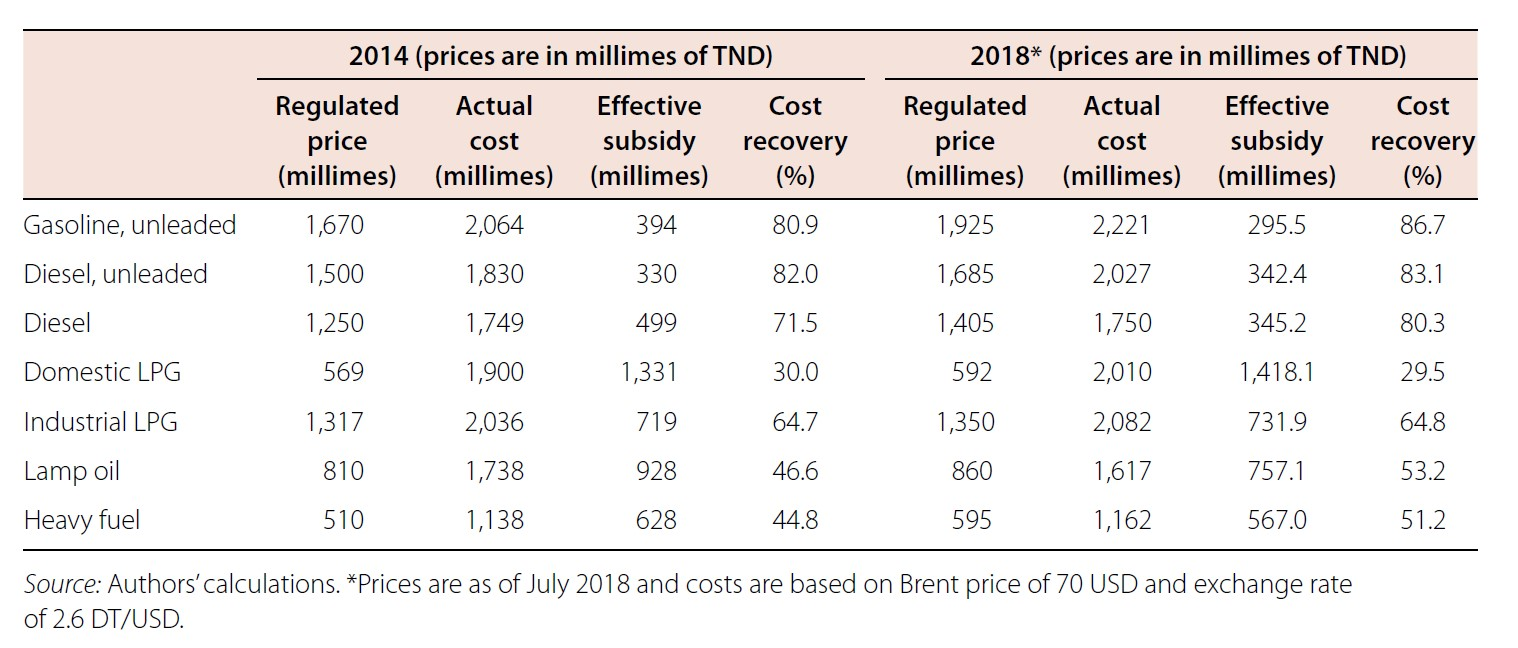
\includegraphics{Images/Composition of fuel subsidies by product.jpg}

Fig.X : Composition of fuel subsidies product (source :
\textcite{tunisia2020})

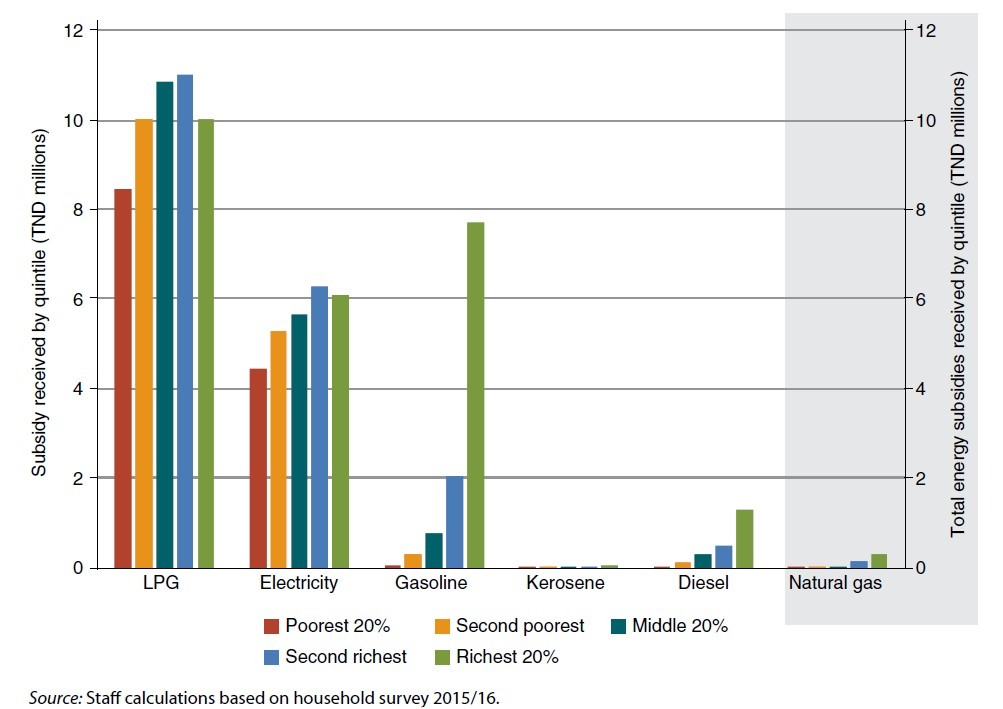
\includegraphics{Images/Energy subsdies received by welfare quintile.jpg}

Fig.X : Energy subsidies received by welfare quintile, 2015/16 (TND
millions) (source : \textcite{tunisia2020})

\hypertarget{climate-policy}{%
\subsection{Climate policy}\label{climate-policy}}

\hypertarget{carbon-tax}{%
\subsubsection{Carbon tax}\label{carbon-tax}}

\hypertarget{energy-subsidy}{%
\subsubsection{Energy subsidy}\label{energy-subsidy}}

Subsidies are defined by \textcite{demoor1997} as \emph{`any measure
that keeps prices for consumers below the market level or keeps prices
for producers above the market level or that reduces costs for consumers
and producers by giving direct or indirect support'}. Energy subsidies
are a common policy. Their amount is estimated at \$4.7 trillion in 2015
as pointed out \textcite{coady2019}, which is equivalent to 6.3 percent
of Gross Domestic Product . Energy subsidies fluctuate depending on the
price of the energy products. From the database of the International
Energy Agency, we can notice that the fossil fuel subsidies have
\href{https://www.iea.org/topics/energy-subsidies}{fallen by 42 percent
between 2019 and 2020} due to the drop of fuel prices.

The energy subsidies are very present in the Middle East, North Africa,
Afghanistan and Pakistan region (MENAP). According to
\textcite{coady2019}, MENAP is the fourth region in absolute terms,
which subsidized the most energy in 2015. Nevertheless, in relative
terms, MENAP is the second, if we take into account the percent of its
GDP. The prevalence of energy subsidies in MENAP can be explained by the
post-par period. These energy subsidies were introduced, after the
decolonization, in Middle East and North Africa region (MENA) in order
to stabilize prices and then, became a social protection system
\autocite{verme2017}.

\textcite{fattouh2013} emphasize three positive aspects of the energy
subsidies that we saw above :

\begin{itemize}
\item
  The energy subsidies enhance the incomes of the poorest part of the
  population. It constitute a core part of the welfare system in the
  MENA.
\item
  The energy subsidies help to reduce production costs and to strengthen
  competitiveness of local firms. Energy subsidies are a tool for
  industrialization and diversification policy.
\item
  The regulation of energy prices is used to control inflation and
  stabilize prices.
\end{itemize}

Reducing energy subsidies may improve economic welfare and reduce
emissions \autocites[ ]{aldy2013}[ ]{coady2019}{hahn2021}.
\textcite{fattouh2013} also highlight unintended consequences of energy
subsidies :

\begin{itemize}
\tightlist
\item
  Energy subsidies raise energy intensity of GDP and reduce energy
  efficiency rates. Low energy pricing favors the growth of
  energy-intensive industries and discourage the firms from minimizing
  energy costs. Fig. X below shows that many energy-intensive countries
  have also high fossil fuel subsidies as a proportion of their GDP.
\item
  Energy subsidies distort consumption. Indeed, they cause a fast growth
  in consumption of primary fuels and electricity. According to
  \textcite{fattouh2013}, between 1980 to 2008, the total energy
  consumption in MENA grew more than 5\% annually.
\item
  Energy subsidies distort investments. The weak implementation of
  subsidies provoke underinvestment in energy sectors, where the
  subsidies do not entirely compensate the energy companies. Therefore,
  end users receive a low quality service.
\item
  Energy subsides cause fuel shortages because of low prices. The
  smuggling across borders is also favored by the price differences
  between countries.
\item
  Non-targeted subsidies create inequities between social groups (see
  fig.~X. above).
\end{itemize}

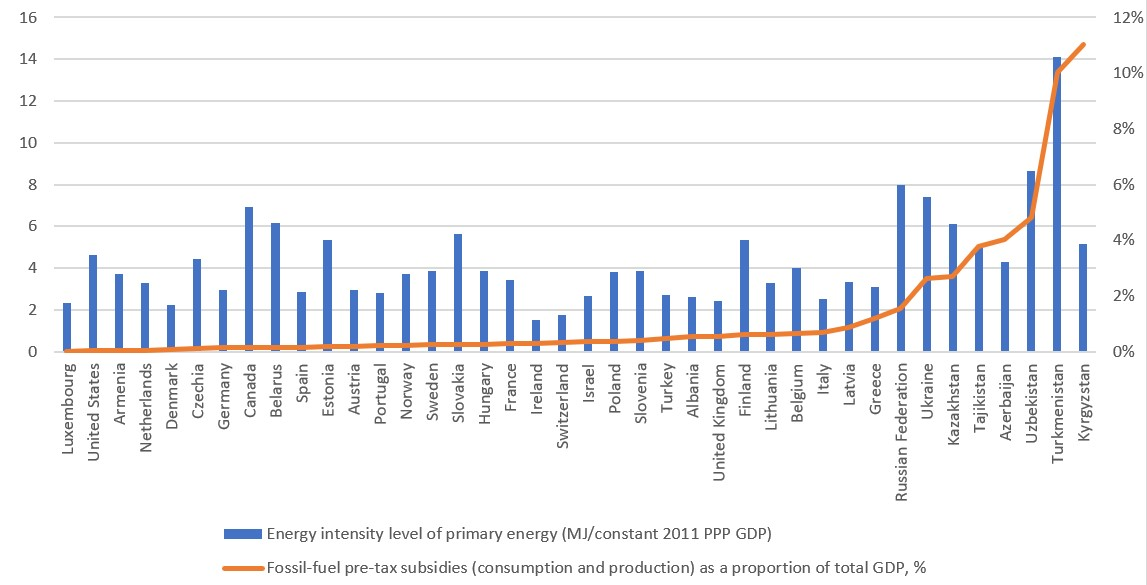
\includegraphics{Images/Subsidies - energy intensity.jpg}

Fig.X : Energy subsidies and energy intensities by country in 2017 (data
: SDG indicators for United Nations Economic Commission for Europe)

\hypertarget{recycle-of-gouvernment-income-for-tax-lucia}{%
\subsubsection{Recycle of gouvernment income for tax
(Lucia)}\label{recycle-of-gouvernment-income-for-tax-lucia}}

Tax redistribution is the mechanism that allows the government to return
to the private economy the revenues that are produced by the instrument
\autocite{goulder}. There are many ways in which this redistribution can
operate. It can be presented as a lump-sum transfer to households and
firms, or as a reduction of taxes that introduce a deformation into the
economy as is the case of the labor tax.

\hypertarget{methodology}{%
\section{Methodology}\label{methodology}}

\hypertarget{threeme-model-bee}{%
\subsection{ThreeME model (Bee)}\label{threeme-model-bee}}

The ThreeME model is a hybrid neo-Keynesian Computable General
Equilibrium model (1), which had to be adaptated and calibrated on
Tunisian data (2).

\hypertarget{a-hybrid-neo-keynesian-computable-general-equilibrium-model}{%
\subsubsection{A hybrid neo-Keynesian Computable General Equilibrium
model}\label{a-hybrid-neo-keynesian-computable-general-equilibrium-model}}

The \href{https://github.com/fosem/ThreeME_V3-open}{open source} ThreeME
model has been developped since 2008 by OFCE (French Economic
Observatory), ADEME (French Environment and Energy Management Agency)
and NEO (Netherlands Economic Observatory). ThreeME is a Computable
General Equilibrium Model (CGEM), with neo-Keynesian features and a
hybrid structure.

ThreeME combines several features \autocites[
]{callonnec2013}{callonnec2021} :

\begin{itemize}
\tightlist
\item
  ThreeME is a Computable General Equilibrium Model (CGEM), which takes
  into account the interactions and feedbacks between supply and demand
  (see Fig.X). Demand defines supply and in return, supply determines
  demand through the production factor incomes.
\end{itemize}

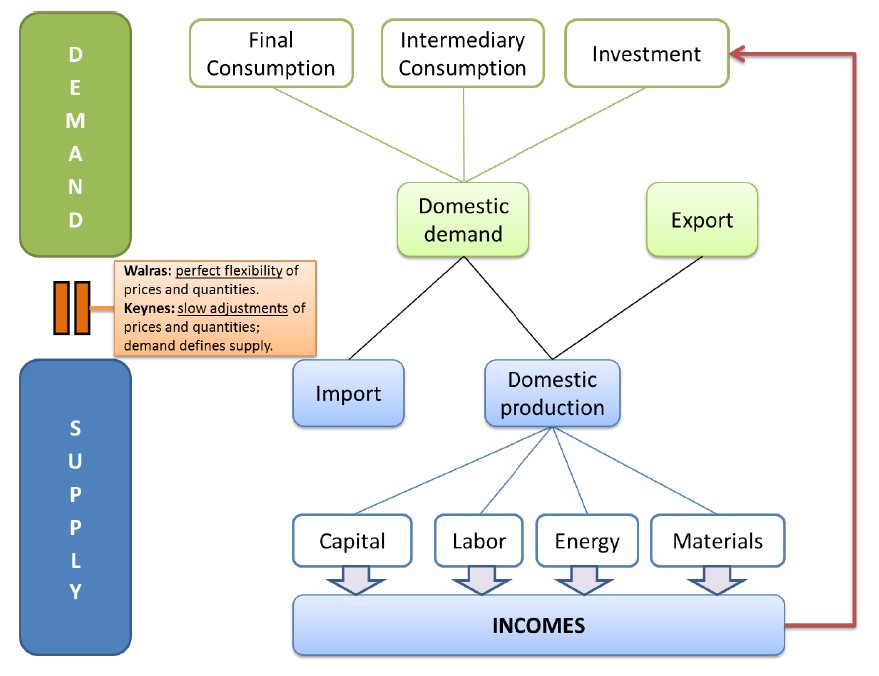
\includegraphics{Images/Architecture of a CGEM.jpg}

Fig.X : Architecture of CGEM (source : \textcite{callonnec2013})

\begin{itemize}
\item
  ThreeME is a CGEM of neo-Keynesian inspiration. ThreeME differs from
  Walrasian CGEM in its dynamics and its transition to the long run.
  Instead of perfect flexibility hypothesis, prices and quantities
  slowly adjust, because of uncertainties, adjustment costs or temporal
  boundaries. Prices do not clear supply and demands and market
  imperfections are also included in the model. Consequently, there are
  disequilibrium between supply and demand. For instance, involuntary
  unemployment is possible.
\item
  The high sectoral disaggregation is a way to describe the transfers of
  activity from a sector to another. The ThreeME model allows to track
  sectoral changes in investment, employment or energy consumption.
\item
  ThreeME is a hybrid model which combines top-down and bottom-up
  modelling. On one side, the general equilibrium effets are
  represented. On the other side, the energy disaggregation allows for
  the analysis of the energy production and consumption. The trade-offs
  between energy and other production factors and between several energy
  consumptions are included in the model.
\end{itemize}

\hypertarget{threeme-model-tunisia-adaptation-for-a-little-country-in-development}{%
\subsubsection{ThreeMe model Tunisia : Adaptation for a little country
in
development}\label{threeme-model-tunisia-adaptation-for-a-little-country-in-development}}

ThreeME has already been adapted to Mexico by \textcite{landarivera2016}
and to Indonesia by \textcite{reynes2017}. The adaptation of ThreeME to
Tunisia has been founded on consultation with Tunisian experts and other
stakeholders. Indeed, the sectoral disaggregation was validated by
Tunisian stakeholders. At the end, 21 sectors and 18 products were
chosen (see Fig.X). The tax structure is based on the supply and use
table (SUT) of the national accounts.

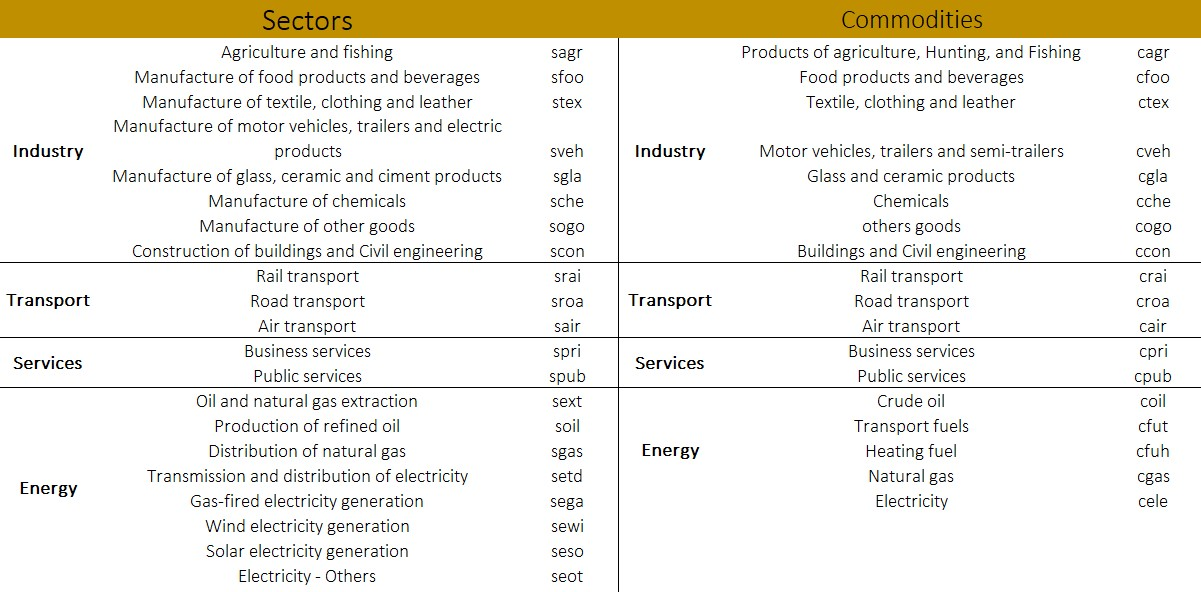
\includegraphics{Images/Sectoral disaggregation.jpg}

Fig.X : Sectoral disaggregation

The required data are economic data from national accounts, in
particular from Input-Output Tables (IOTs), physical data from energy
balance and detailed tax data by product. These data were collected from
Tunisian institutions, in particular ANME (National Agency for Energy
Management), INS (National Institute of statistics), ONE (National
Energy Observatory), STEG (Tunisian Company of Electricity and Gas),
ITCEQ (Tunisian Institute of Competitiveness and Quantitative Studies),
Ministry of Energy, Mines and Energy Transition and the Ministry of
Economic Development, Investment and International Cooperation.

\hypertarget{description-of-scenario-lucia}{%
\subsection{Description of scenario
(Lucia)}\label{description-of-scenario-lucia}}

with/without redistribution? *Voir si peut être on déplace cette partie

We work on six different scenarios that simulate the implementation of
six alternative environmental policies.

Scenario 1 : Implementation of a carbon tax from 2021 without
redistribution of the revenues of the tax in the economy - they are used
to reduce public debt.

Scenario 2 : Carbon tax with recycling of revenues that are redirected
to the Energy Transition Fund. In fact, a part is given back to
households and a portion is devoted to ``non-polluting'' businesses.

Scenario 3 : Fossil fuels subsidies removal (without recycling).

Scenario 4 : Fossil fuels subsidies removal (with recycling). A part is
given back to households and a portion is given to enterprises in
proportion to the employment of each sector in the total salaried labor
force.

Scenario 5 : Significant penetration of Renewable Energies in the
electrical mix (80\% by 2050)

Scenario 6 : Combination of scenarios 2, 4 and 5.

\hypertarget{tax-carbon-scenario}{%
\subsubsection{Tax carbon scenario}\label{tax-carbon-scenario}}

Avant 2030, le niveau de la TC est calculé de façon a couvrir 100\% des
besoins du FTE Il passe de 1.1 à 9 DT/tCO2 Après 2030, la trajectoire de
la TC est définie de façon à atteindre les objectifs de réduction
d'émission à 2050 D'après les hypothèse des substitutions retenues dans
ThreeME, l'atteinte d'un factor 5 en 2050 par rapport au niveau de 2020
nécessite une hause régulière de 9 DT/tCO2 à 372 DT/ tCO2. En plus de la
TC des signaux prix ont été introduits afin d'atteindre les objectifs de
consommations d'énergie par source

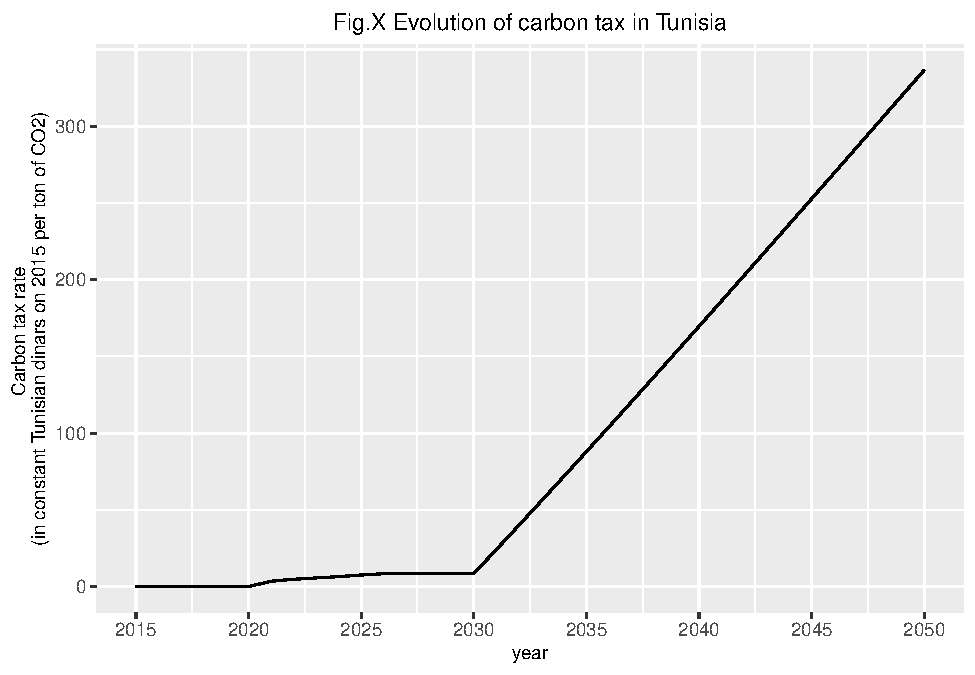
\includegraphics{Modele-ThreeMe-Tunisie_Sequeira_Valilou_Wang_files/figure-latex/unnamed-chunk-6-1.pdf}

\hypertarget{energy-subsidy-removal-scenario}{%
\subsubsection{Energy subsidy removal
scenario}\label{energy-subsidy-removal-scenario}}

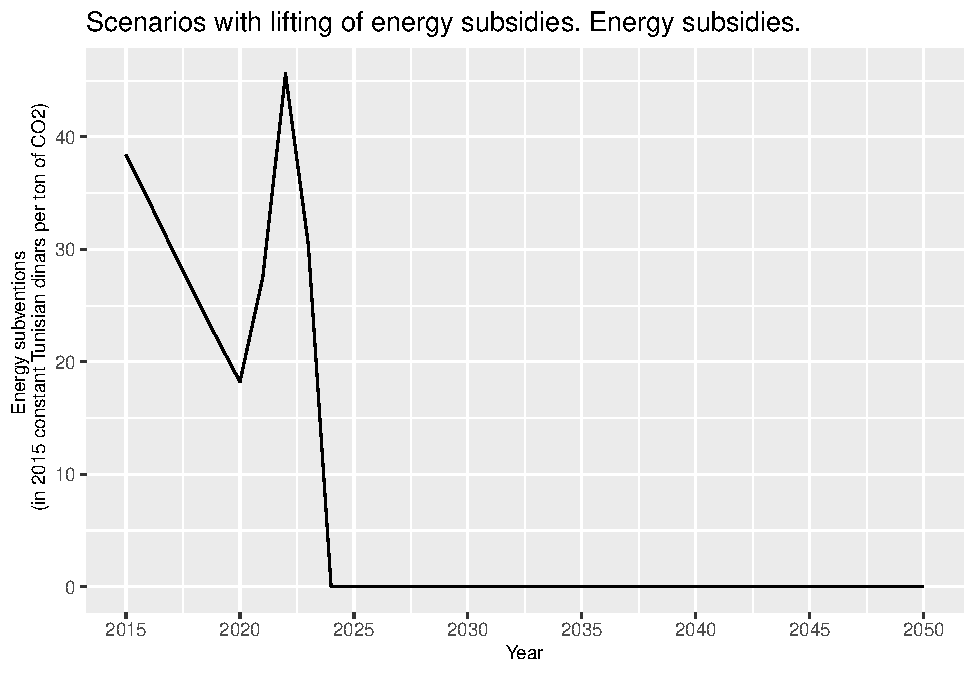
\includegraphics{Modele-ThreeMe-Tunisie_Sequeira_Valilou_Wang_files/figure-latex/unnamed-chunk-7-1.pdf}

\hypertarget{renewable-energy-scenario}{%
\subsubsection{Renewable energy
scenario}\label{renewable-energy-scenario}}

\hypertarget{national-low-carbon-strategy-scenario}{%
\subsubsection{National Low-Carbon Strategy
scenario}\label{national-low-carbon-strategy-scenario}}

\hypertarget{choice-of-evaluation-indicators}{%
\subsection{Choice of evaluation
indicators}\label{choice-of-evaluation-indicators}}

\hypertarget{data-structure}{%
\subsubsection{Data structure}\label{data-structure}}

All the indicators used in the analysis are in exact hat algebra,
meaning the proportional variation to Baseline scenario. time scale of
data key indicator: two dimensions economy and environnement

\hypertarget{kaya-identity-jin}{%
\subsubsection{Kaya identity (Jin)}\label{kaya-identity-jin}}

The Kaya identity, firstly proposed by \autocite{kaya1989}, is an
identity where the total emission of carbon dioxide can be explained by
four product driving forces as population, Gross Domestic Product (GDP)
per capita, enerny intensity over GDP and carbon intensity over energy
consumption \autocite{kayaide2021}. It is expressed in the form:

\[ C = POP \cdot \frac{GDP}{POP} \cdot \frac{TEC}{GDP} \cdot \frac{C}{TEC} \tag{1}\]

where:

\begin{itemize}
\tightlist
\item
  POP is global population;
\item
  GDP is gross domestic product;
\item
  TEC is total energy consumption;
\item
  C is total emission of carbon dioxide;
\end{itemize}

And:

\begin{itemize}
\tightlist
\item
  GDP/POP is GDP per capita describing the economical activities within
  a period;
\item
  TEC/GDP is energy intensity;
\item
  C/TEC is carbon intensity;
\end{itemize}

In this study, we introduced an extension of Kaya identity to explain
how different driving forces influenced the total emission for different
scenarios. Firstly, a extended Kaya identity is used to analysis
CO\textsubscript{2} emission with the aggregated factors, then we couple
with Logarithmic Mean Divisia Index (LMDI) method to decomposite
CO\textsubscript{2} emission at the sectorial level.

We modified the function of Kaya identity mentioned above to adapt our
model assumption, where we integrated a new driving force, named economy
structure, to decomposite emissions driving force at sectorial level.
The five economic sectors considered in ThreeME Tunisia model are:
Industry and Agriculture, Service, Transportation, Energy Transformation
and Electricity. However, we did not take population into consideration
because its increasing rate remains still over time for all our
scenarios and is considered as an exogenous variable in ThreeME model.

Therefore, the CO\textsubscript{2} emission can be written as:

\[  C_{tot} = \Sigma C_{i} = \Sigma( VA \cdot \frac{VA_{i}}{VA} \cdot \frac{EC_{i}}{VA_{i}} \cdot \frac{CE_{i}}{EC_{i}} )=  \Sigma( V \cdot S_{i} \cdot E_{i} \cdot I_{i}) \tag{2}\]
where C\textsubscript{tot} is overall CO\textsubscript{2} emission,
C\textsubscript{i} is CO\textsubscript{2} emission of economic sector i,
VA is total added value, VA\textsubscript{i} is added value of sector i,
EC\textsubscript{i} is total energy consumption by sector i,
CE\textsubscript{i} is CO\textsubscript{2} emission arising from sector
i. According to equation 8, total CO\textsubscript{2} emission can be
explained by four driving forces, including one aggregated indicator,
overall economic activities V, and three sectorial indicators, share of
total added value of sector i S\textsubscript{i}, energy intensity over
added value of sector i E\textsubscript{i} and carbon intensity over
energy consumption of sector i I\textsubscript{i}. Especially,
S\textsubscript{i} can be interpreted as economy structure of Tunisia,
\textcite{grubb2015} and \textcite{kanitkar2015} found that for a
developing country, this term could be a key variable determining the
future emissions pathway.

The effects of driving forces can be expressed in two ways:
multiplicative and additive form, where multiplicative deviation
\(D_{tot}\) is the ratio of total CO\textsubscript{2} emission between
policy scenario and baseline scenario (equation 3), and additive
deviation \(\Delta C_{tot}\) is the difference of total
CO\textsubscript{2} emission (equation 4). The two expressions are shown
below:

\[ D_{tot} =\frac{C_{2}}{C_{0}} = \Pi(\frac{V_{2}}{V_{0}} \cdot \frac{S_{2,i}}{S_{0,i}} \cdot \frac{E_{2,i}}{E_{0,i}}  \cdot \frac{I_{2,i}}{I_{0,i}}) = D_{V}  \cdot  D_{S} \cdot D_{E} \cdot D_{I} = D_{V}  \cdot \Pi ( D_{S_{i}} \cdot D_{E_{i}} \cdot D_{I_{i}}) \tag{3}\]

\[ \Delta C_{tot} = C_{2} - C_{0} = \Delta C_{V} + \Delta C_{S} + \Delta C_{E} + \Delta C_{I} = \Delta C_{V} + \Sigma( \Delta C_{S_{i}} + \Delta C_{E_{i}} + \Delta C_{I_{i}}) \tag{4}\]
where subscript \(tot\) represents overall change of emission, subscript
0 and 2 mean baseline scenario and policy scenario respectively. Hence
we obtain the index \(D_{V}\), \(D_{S}\), \(D_{E}\) and \(D_{I}\),
meaning the deviation of emissions due to change of overall economic
activities, economy structure, energy intensity and carbon intensity,
while \(\Delta C_{V}\), \(\Delta C_{S}\), \(\Delta C_{E}\) and
\(\Delta C_{I}\) depict the difference of emissions related to change of
driving forces.

Now we expect to identify the effect of each driving force at a
sectorial level, to do this, we used a LMDI method proposed by
\textcite{ang1997} and \textcite{ang2005}. For multiplicative form, we
have:

\[ D_{X} = exp ( \Sigma \frac{(C_{2,i}-C_{0,i})/(lnC_{2,i}-lnC_{0,i})}{(C_{2}-C_{0})/(lnC_{2}-lnC_{0})} \cdot ln \frac{X_{2,(i)}}{X_{0,(i)}} ) \tag{11}\]
\[ \Delta C_{X} =  \Sigma (\frac{C_{2,i}-C_{0,i}}{lnC_{2,i}-lnC_{0,i}} \cdot ln\frac{X_{2,(i)}}{X_{0,(i)}}) \tag{12} \]
where \(C_{2}\) is total emission of policy scenario, \(C_{0}\) is total
emission of baseline, \(C_{2,i}\) is emission of policy scenario arising
from sector i, \(C_{0,i}\) is emission of baseline arising from sector
i, \(D_{X}\) and \(\Delta C_{X}\) represent multiplicative and additive
index of driving force \(X\), \(X_{2,(i)}\) is value of driving force
\(X\) of policy scenario for sector i, \(X_{0,(i)}\) is value of driving
force \(X\) of baseline for sector i.

\hypertarget{results-et-discussions}{%
\section{Results et discussions}\label{results-et-discussions}}

In this section we will analyse the results obtained for the different
scenarios for the different variables taken into account.

\hypertarget{importance-of-redistribution-lucia}{%
\subsection{Importance of redistribution
(Lucia)}\label{importance-of-redistribution-lucia}}

Here we will analyse the influence of the redistribution of both the tax
and the removed energy subsidy. We will observe the impact of the
redistribution on the economical and environmental aspects. We will
focus on GDP variation and unemployment when it comes to the economical
aspect and we will analyse the evolution of emissions for the
environmental aspect.

Firstly, we will analyse the redistribution of the carbon tax. The
figure below show the variation in GDP in relation to the baseline for
both the scenarios carbon tax with and without redistribution. We
observe that the evolution of the curves is opposite and symmetric in
relation to the x-axis, the scenario with redistribution showing a
marked increase in GDP.

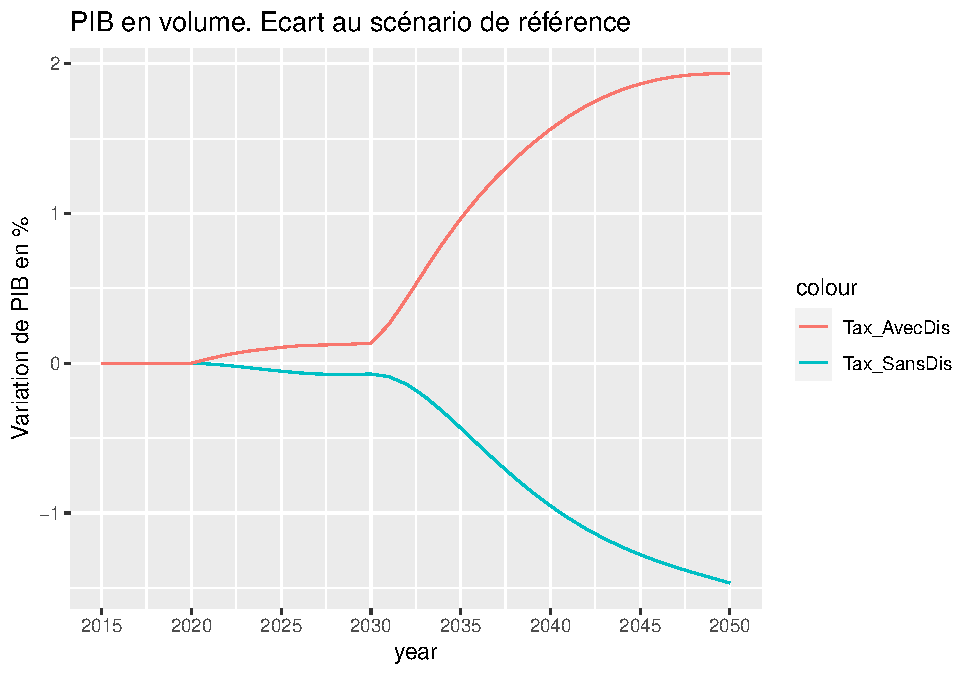
\includegraphics{Modele-ThreeMe-Tunisie_Sequeira_Valilou_Wang_files/figure-latex/unnamed-chunk-8-1.pdf}

Then when we analyse the \emph{level of employment} we can see that the
redistribution operates an increase on it in relation to the baseline,
when the scenario of a carbon tax without redistribution produce a
decrease in the level of employment. That is consistent with the fact
that the

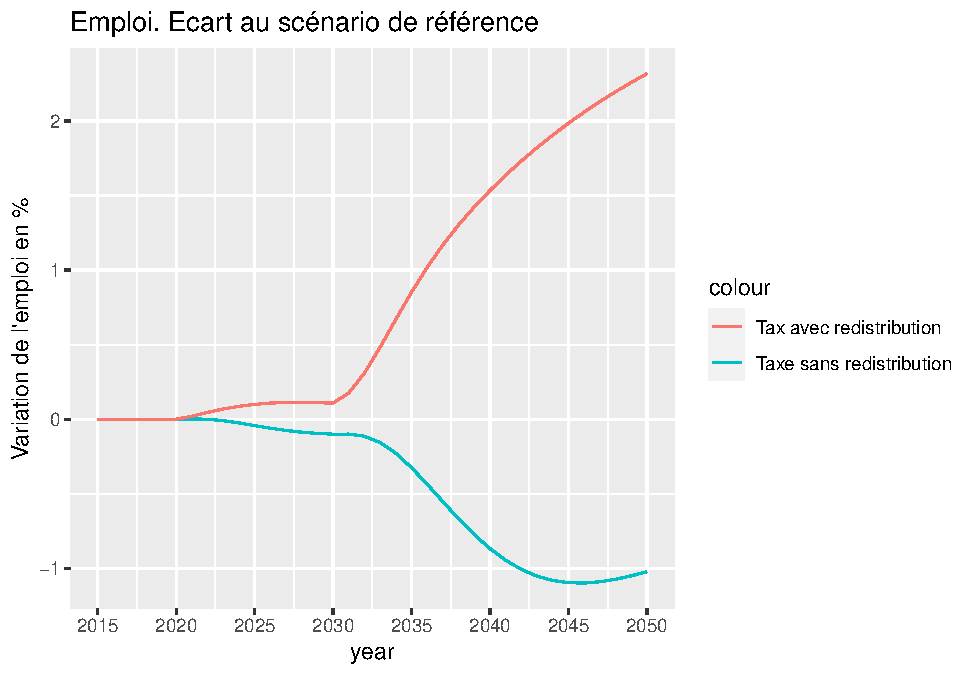
\includegraphics{Modele-ThreeMe-Tunisie_Sequeira_Valilou_Wang_files/figure-latex/unnamed-chunk-9-1.pdf}

emissions

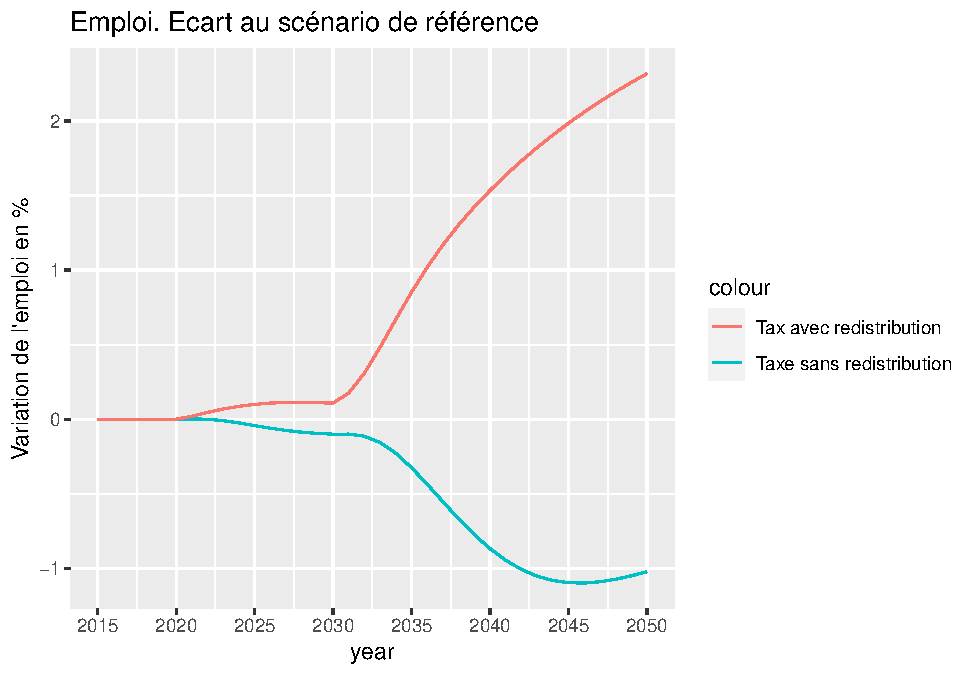
\includegraphics{Modele-ThreeMe-Tunisie_Sequeira_Valilou_Wang_files/figure-latex/unnamed-chunk-10-1.pdf}

PIB

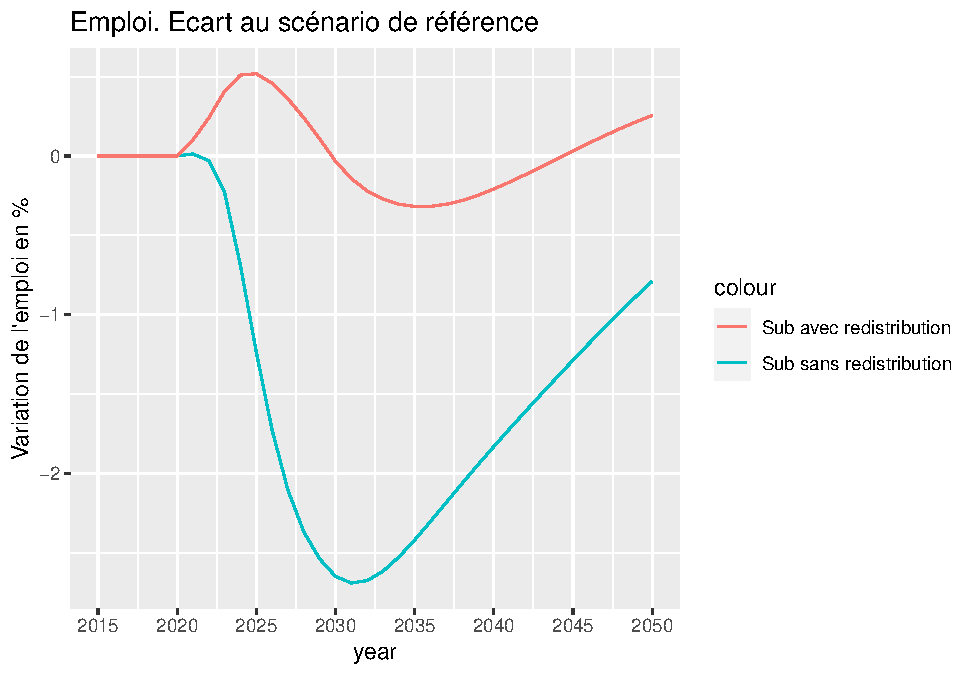
\includegraphics{Modele-ThreeMe-Tunisie_Sequeira_Valilou_Wang_files/figure-latex/unnamed-chunk-11-1.pdf}

chomage :

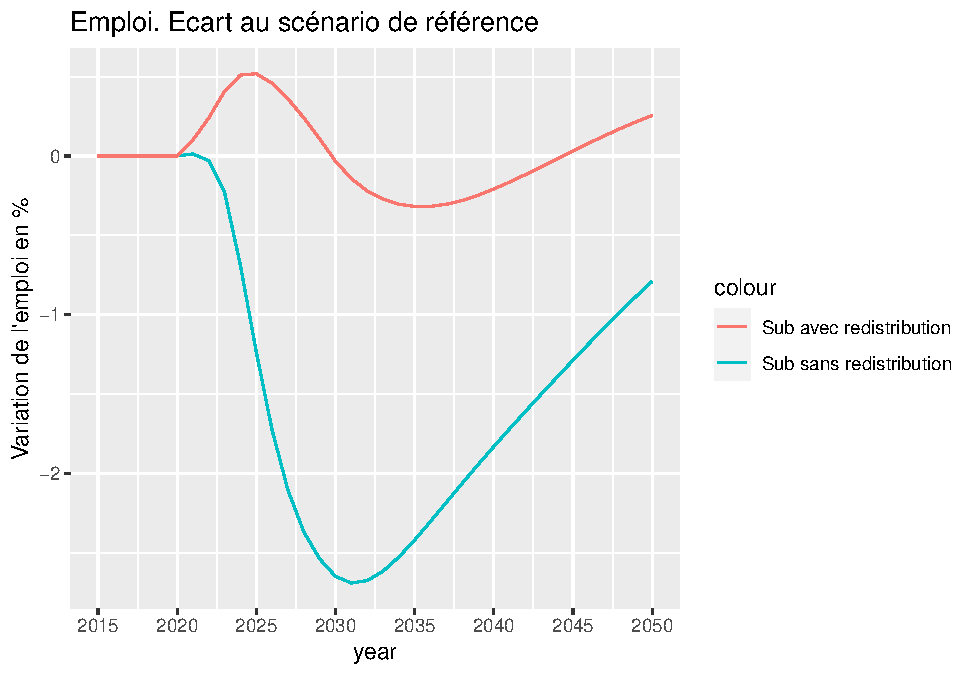
\includegraphics{Modele-ThreeMe-Tunisie_Sequeira_Valilou_Wang_files/figure-latex/unnamed-chunk-12-1.pdf}

Il peut être intéressant de faire un commentaire sur le salaire brut

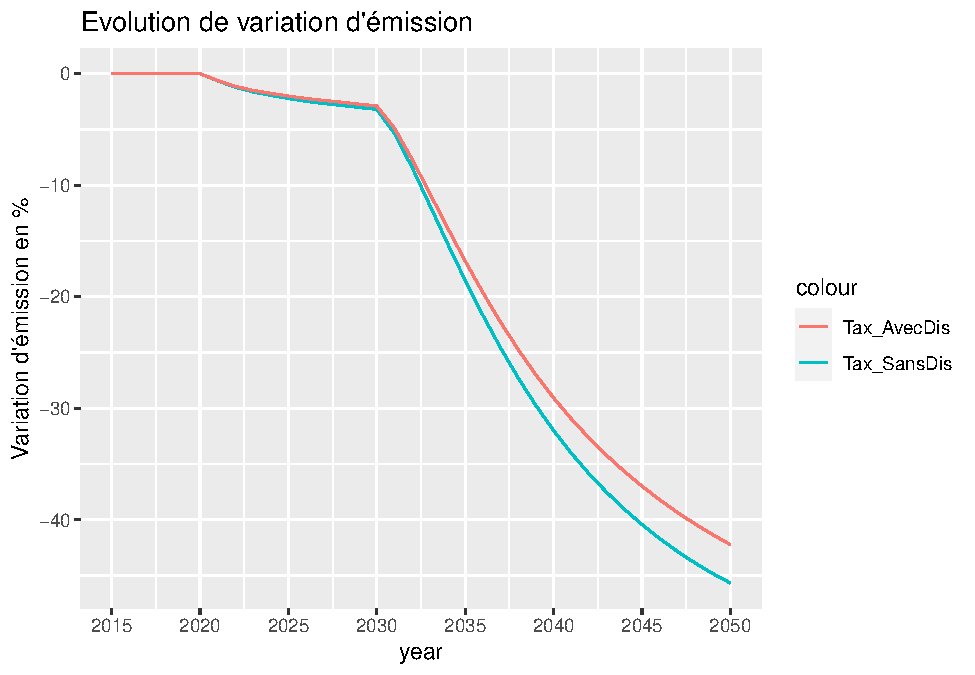
\includegraphics{Modele-ThreeMe-Tunisie_Sequeira_Valilou_Wang_files/figure-latex/unnamed-chunk-13-1.pdf}

émissions :

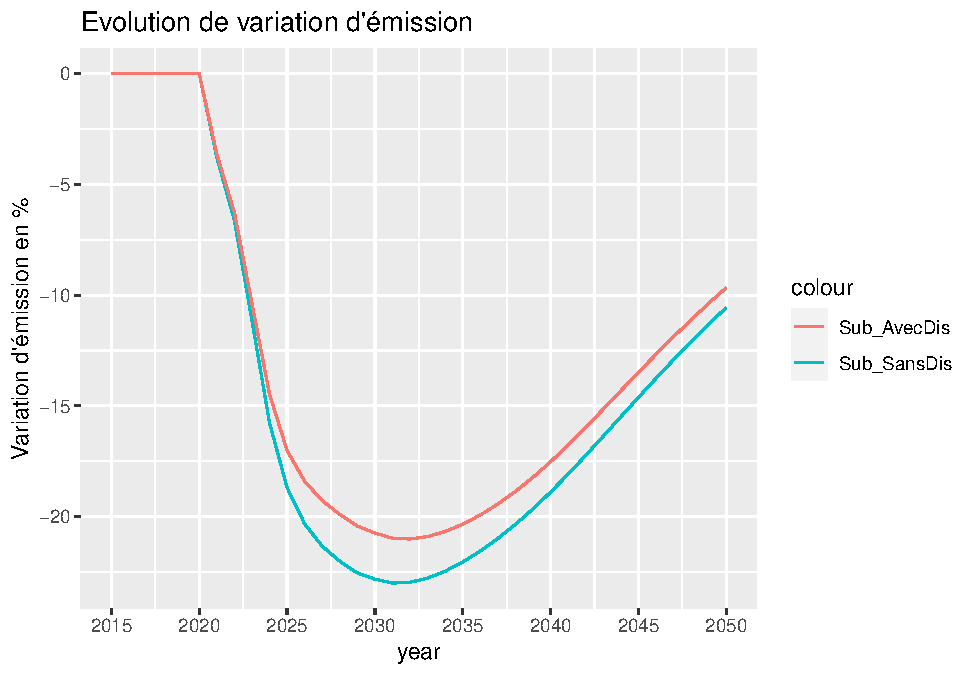
\includegraphics{Modele-ThreeMe-Tunisie_Sequeira_Valilou_Wang_files/figure-latex/unnamed-chunk-14-1.pdf}

Tableau Taxe sans redistribution

\begin{Shaded}
\begin{Highlighting}[]
\NormalTok{tablename }\OtherTok{\textless{}{-}} \FunctionTok{c}\NormalTok{(}\StringTok{"GDP in volume"}\NormalTok{,}\StringTok{"Household consumption"}\NormalTok{,}\StringTok{"Investment"}\NormalTok{,}\StringTok{"Exports"}\NormalTok{,}\StringTok{"Imports"}\NormalTok{,}\StringTok{"Household disposable income"}\NormalTok{,}\StringTok{"Household consumption price index"}\NormalTok{,}\StringTok{"production price index"}\NormalTok{,}\StringTok{"Added value price index"}\NormalTok{,}\StringTok{"Intermediate consumption price index"}\NormalTok{,}\StringTok{"Export price index"}\NormalTok{,}\StringTok{"Import price index"}\NormalTok{,}\StringTok{"Gross nominal wage"}\NormalTok{,}\StringTok{"Real cost of labor"}\NormalTok{,}\StringTok{"Wage employment rate (in thousands)"}\NormalTok{,}\StringTok{"Unemployment rate (in point)"}\NormalTok{,}\StringTok{"Trade balance (in point of GDP)"}\NormalTok{,}\StringTok{"Public budget balance (in points of GDP)"}\NormalTok{,}\StringTok{"Public debt (in points of GDP)"}\NormalTok{, }\StringTok{"CO2 emissions"}\NormalTok{)}

\NormalTok{Table\_Macro\_CT }\OtherTok{\textless{}{-}}\NormalTok{ S1\_Macro[}\FunctionTok{c}\NormalTok{(}\StringTok{"2021"}\NormalTok{,}\StringTok{"2025"}\NormalTok{,}\StringTok{"2030"}\NormalTok{,}\StringTok{"2035"}\NormalTok{,}\StringTok{"2040"}\NormalTok{,}\StringTok{"2045"}\NormalTok{,}\StringTok{"2050"}\NormalTok{),}\DecValTok{1}\SpecialCharTok{:}\DecValTok{20}\NormalTok{]}
\NormalTok{Table\_Macro\_CT }\OtherTok{\textless{}{-}} \FunctionTok{t}\NormalTok{(Table\_Macro\_CT)}
\NormalTok{Table\_Macro\_CT }\OtherTok{\textless{}{-}} \FunctionTok{round}\NormalTok{(Table\_Macro\_CT,}\AttributeTok{digits =} \DecValTok{2}\NormalTok{)}
\FunctionTok{row.names}\NormalTok{(Table\_Macro\_CT) }\OtherTok{\textless{}{-}}\NormalTok{ tablename}

\FunctionTok{kable}\NormalTok{(Table\_Macro\_CT, }\AttributeTok{booktabs =}\NormalTok{ T, }\AttributeTok{longtable =}\NormalTok{ T, }\AttributeTok{linesep =} \StringTok{""}\NormalTok{, }\AttributeTok{caption =} \StringTok{"Macroeconomic impacts of Carbon tax scenario in percent deviation to Baseline"}\NormalTok{) }\SpecialCharTok{\%\textgreater{}\%} 
\FunctionTok{kable\_styling}\NormalTok{(}\AttributeTok{latex\_options =} \FunctionTok{c}\NormalTok{(}\StringTok{"striped"}\NormalTok{,}\StringTok{"hover"}\NormalTok{,}\StringTok{"repeat\_header"}\NormalTok{), }\AttributeTok{full\_width =}\NormalTok{ T) }\SpecialCharTok{\%\textgreater{}\%} 
\FunctionTok{row\_spec}\NormalTok{(}\DecValTok{0}\NormalTok{, }\AttributeTok{bold =}\NormalTok{ T)}
\end{Highlighting}
\end{Shaded}

Tableau Taxe avec redistribution

\begin{Shaded}
\begin{Highlighting}[]
\NormalTok{tablename }\OtherTok{\textless{}{-}} \FunctionTok{c}\NormalTok{(}\StringTok{"GDP in volume"}\NormalTok{,}\StringTok{"Household consumption"}\NormalTok{,}\StringTok{"Investment"}\NormalTok{,}\StringTok{"Exports"}\NormalTok{,}\StringTok{"Imports"}\NormalTok{,}\StringTok{"Household disposable income"}\NormalTok{,}\StringTok{"Household consumption price index"}\NormalTok{,}\StringTok{"production price index"}\NormalTok{,}\StringTok{"Added value price index"}\NormalTok{,}\StringTok{"Intermediate consumption price index"}\NormalTok{,}\StringTok{"Export price index"}\NormalTok{,}\StringTok{"Import price index"}\NormalTok{,}\StringTok{"Gross nominal wage"}\NormalTok{,}\StringTok{"Real cost of labor"}\NormalTok{,}\StringTok{"Wage employment rate (in thousands)"}\NormalTok{,}\StringTok{"Unemployment rate (in point)"}\NormalTok{,}\StringTok{"Trade balance (in point of GDP)"}\NormalTok{,}\StringTok{"Public budget balance (in points of GDP)"}\NormalTok{,}\StringTok{"Public debt (in points of GDP)"}\NormalTok{, }\StringTok{"CO2 emissions"}\NormalTok{)}

\NormalTok{Table\_Macro\_CT }\OtherTok{\textless{}{-}}\NormalTok{ S2\_Macro[}\FunctionTok{c}\NormalTok{(}\StringTok{"2021"}\NormalTok{,}\StringTok{"2025"}\NormalTok{,}\StringTok{"2030"}\NormalTok{,}\StringTok{"2035"}\NormalTok{,}\StringTok{"2040"}\NormalTok{,}\StringTok{"2045"}\NormalTok{,}\StringTok{"2050"}\NormalTok{),}\DecValTok{1}\SpecialCharTok{:}\DecValTok{20}\NormalTok{]}
\NormalTok{Table\_Macro\_CT }\OtherTok{\textless{}{-}} \FunctionTok{t}\NormalTok{(Table\_Macro\_CT)}
\NormalTok{Table\_Macro\_CT }\OtherTok{\textless{}{-}} \FunctionTok{round}\NormalTok{(Table\_Macro\_CT,}\AttributeTok{digits =} \DecValTok{2}\NormalTok{)}
\FunctionTok{row.names}\NormalTok{(Table\_Macro\_CT) }\OtherTok{\textless{}{-}}\NormalTok{ tablename}

\FunctionTok{kable}\NormalTok{(Table\_Macro\_CT, }\AttributeTok{booktabs =}\NormalTok{ T, }\AttributeTok{longtable =}\NormalTok{ T, }\AttributeTok{linesep =} \StringTok{""}\NormalTok{, }\AttributeTok{caption =} \StringTok{"Macroeconomic impacts of Carbon tax scenario in percent deviation to Baseline"}\NormalTok{) }\SpecialCharTok{\%\textgreater{}\%} 
\FunctionTok{kable\_styling}\NormalTok{(}\AttributeTok{latex\_options =} \FunctionTok{c}\NormalTok{(}\StringTok{"striped"}\NormalTok{,}\StringTok{"hover"}\NormalTok{,}\StringTok{"repeat\_header"}\NormalTok{), }\AttributeTok{full\_width =}\NormalTok{ T) }\SpecialCharTok{\%\textgreater{}\%} 
\FunctionTok{row\_spec}\NormalTok{(}\DecValTok{0}\NormalTok{, }\AttributeTok{bold =}\NormalTok{ T)}
\end{Highlighting}
\end{Shaded}

Tableau subvention sans redistribution

\begin{Shaded}
\begin{Highlighting}[]
\NormalTok{tablename }\OtherTok{\textless{}{-}} \FunctionTok{c}\NormalTok{(}\StringTok{"GDP in volume"}\NormalTok{,}\StringTok{"Household consumption"}\NormalTok{,}\StringTok{"Investment"}\NormalTok{,}\StringTok{"Exports"}\NormalTok{,}\StringTok{"Imports"}\NormalTok{,}\StringTok{"Household disposable income"}\NormalTok{,}\StringTok{"Household consumption price index"}\NormalTok{,}\StringTok{"production price index"}\NormalTok{,}\StringTok{"Added value price index"}\NormalTok{,}\StringTok{"Intermediate consumption price index"}\NormalTok{,}\StringTok{"Export price index"}\NormalTok{,}\StringTok{"Import price index"}\NormalTok{,}\StringTok{"Gross nominal wage"}\NormalTok{,}\StringTok{"Real cost of labor"}\NormalTok{,}\StringTok{"Wage employment rate (in thousands)"}\NormalTok{,}\StringTok{"Unemployment rate (in point)"}\NormalTok{,}\StringTok{"Trade balance (in point of GDP)"}\NormalTok{,}\StringTok{"Public budget balance (in points of GDP)"}\NormalTok{,}\StringTok{"Public debt (in points of GDP)"}\NormalTok{, }\StringTok{"CO2 emissions"}\NormalTok{)}

\NormalTok{Table\_Macro\_CT }\OtherTok{\textless{}{-}}\NormalTok{ S3\_Macro[}\FunctionTok{c}\NormalTok{(}\StringTok{"2021"}\NormalTok{,}\StringTok{"2025"}\NormalTok{,}\StringTok{"2030"}\NormalTok{,}\StringTok{"2035"}\NormalTok{,}\StringTok{"2040"}\NormalTok{,}\StringTok{"2045"}\NormalTok{,}\StringTok{"2050"}\NormalTok{),}\DecValTok{1}\SpecialCharTok{:}\DecValTok{20}\NormalTok{]}
\NormalTok{Table\_Macro\_CT }\OtherTok{\textless{}{-}} \FunctionTok{t}\NormalTok{(Table\_Macro\_CT)}
\NormalTok{Table\_Macro\_CT }\OtherTok{\textless{}{-}} \FunctionTok{round}\NormalTok{(Table\_Macro\_CT,}\AttributeTok{digits =} \DecValTok{2}\NormalTok{)}
\FunctionTok{row.names}\NormalTok{(Table\_Macro\_CT) }\OtherTok{\textless{}{-}}\NormalTok{ tablename}

\FunctionTok{kable}\NormalTok{(Table\_Macro\_CT, }\AttributeTok{booktabs =}\NormalTok{ T, }\AttributeTok{longtable =}\NormalTok{ T, }\AttributeTok{linesep =} \StringTok{""}\NormalTok{, }\AttributeTok{caption =} \StringTok{"Macroeconomic impacts of Carbon tax scenario in percent deviation to Baseline"}\NormalTok{) }\SpecialCharTok{\%\textgreater{}\%} 
\FunctionTok{kable\_styling}\NormalTok{(}\AttributeTok{latex\_options =} \FunctionTok{c}\NormalTok{(}\StringTok{"striped"}\NormalTok{,}\StringTok{"hover"}\NormalTok{,}\StringTok{"repeat\_header"}\NormalTok{), }\AttributeTok{full\_width =}\NormalTok{ T) }\SpecialCharTok{\%\textgreater{}\%} 
\FunctionTok{row\_spec}\NormalTok{(}\DecValTok{0}\NormalTok{, }\AttributeTok{bold =}\NormalTok{ T)}
\end{Highlighting}
\end{Shaded}

Tableau subvention avec redistribution

\begin{Shaded}
\begin{Highlighting}[]
\NormalTok{tablename }\OtherTok{\textless{}{-}} \FunctionTok{c}\NormalTok{(}\StringTok{"GDP in volume"}\NormalTok{,}\StringTok{"Household consumption"}\NormalTok{,}\StringTok{"Investment"}\NormalTok{,}\StringTok{"Exports"}\NormalTok{,}\StringTok{"Imports"}\NormalTok{,}\StringTok{"Household disposable income"}\NormalTok{,}\StringTok{"Household consumption price index"}\NormalTok{,}\StringTok{"production price index"}\NormalTok{,}\StringTok{"Added value price index"}\NormalTok{,}\StringTok{"Intermediate consumption price index"}\NormalTok{,}\StringTok{"Export price index"}\NormalTok{,}\StringTok{"Import price index"}\NormalTok{,}\StringTok{"Gross nominal wage"}\NormalTok{,}\StringTok{"Real cost of labor"}\NormalTok{,}\StringTok{"Wage employment rate (in thousands)"}\NormalTok{,}\StringTok{"Unemployment rate (in point)"}\NormalTok{,}\StringTok{"Trade balance (in point of GDP)"}\NormalTok{,}\StringTok{"Public budget balance (in points of GDP)"}\NormalTok{,}\StringTok{"Public debt (in points of GDP)"}\NormalTok{, }\StringTok{"CO2 emissions"}\NormalTok{)}

\NormalTok{Table\_Macro\_CT }\OtherTok{\textless{}{-}}\NormalTok{ S4\_Macro[}\FunctionTok{c}\NormalTok{(}\StringTok{"2021"}\NormalTok{,}\StringTok{"2025"}\NormalTok{,}\StringTok{"2030"}\NormalTok{,}\StringTok{"2035"}\NormalTok{,}\StringTok{"2040"}\NormalTok{,}\StringTok{"2045"}\NormalTok{,}\StringTok{"2050"}\NormalTok{),}\DecValTok{1}\SpecialCharTok{:}\DecValTok{20}\NormalTok{]}
\NormalTok{Table\_Macro\_CT }\OtherTok{\textless{}{-}} \FunctionTok{t}\NormalTok{(Table\_Macro\_CT)}
\NormalTok{Table\_Macro\_CT }\OtherTok{\textless{}{-}} \FunctionTok{round}\NormalTok{(Table\_Macro\_CT,}\AttributeTok{digits =} \DecValTok{2}\NormalTok{)}
\FunctionTok{row.names}\NormalTok{(Table\_Macro\_CT) }\OtherTok{\textless{}{-}}\NormalTok{ tablename}

\FunctionTok{kable}\NormalTok{(Table\_Macro\_CT, }\AttributeTok{booktabs =}\NormalTok{ T, }\AttributeTok{longtable =}\NormalTok{ T, }\AttributeTok{linesep =} \StringTok{""}\NormalTok{, }\AttributeTok{caption =} \StringTok{"Macroeconomic impacts of Carbon tax scenario in percent deviation to Baseline"}\NormalTok{) }\SpecialCharTok{\%\textgreater{}\%} 
\FunctionTok{kable\_styling}\NormalTok{(}\AttributeTok{latex\_options =} \FunctionTok{c}\NormalTok{(}\StringTok{"striped"}\NormalTok{,}\StringTok{"hover"}\NormalTok{,}\StringTok{"repeat\_header"}\NormalTok{), }\AttributeTok{full\_width =}\NormalTok{ T) }\SpecialCharTok{\%\textgreater{}\%} 
\FunctionTok{row\_spec}\NormalTok{(}\DecValTok{0}\NormalTok{, }\AttributeTok{bold =}\NormalTok{ T)}
\end{Highlighting}
\end{Shaded}

\hypertarget{carbon-tax-jin}{%
\subsection{Carbon tax (jin)}\label{carbon-tax-jin}}

As the carbon tax before 2030 stays at a moderate level, the impacts of
this policy are therefore limited, while the significant effects are
observed during the later period from 2030 to 2050 when a much stronger
tax carbon is implemented. The macroeconomic impacts are summarized in
table 1, the results are expressed as percentage deviation from Baseline
scenario.

Generally speaking, the policy of carbon tax with redistribution of
government revenue has a positive impact on Tunisia's economy. Whereas
GDP increases slightly up to 0.13\% with respect to baseline on 2030,
the relatively rapid augmentation is observed from 2030 to 2050. At the
horizon of 2050, it reaches a highest level (+1.93\%) thanks to the
carbon tax policy. In the meantime, social welfare is improved with the
same rhythme as GDP growth, with a higher consumption level (+4.20\%)
and a higher disposable income (+4.17\%) on 2050.

Table.X :Macroeconomic impacts of Carbon tax scenario in \% deviation to
Baseline

An intuitive influence of carbon tax is that the price of internal
market will raise, which is in line with our model output: higher
household consumption price of 9.49\% with 11.33\% and 13.14\% for
production price and intermediate consumption price, respectively. The
increasing cost of household and company will force them to choose the
substitution with less CO2 emissions, thus reducing their cost. The
variation of internal price also has an impact on the competitiveness of
local goods on international market, causing a recession for exportation
and a boost for importation.

It is interesting to note that the implemented policy can alleviate
social poverty to some extent. We observed, for example, the continuous
growth of wage employment. It will then reinforce the acceptability of
the climate policy.

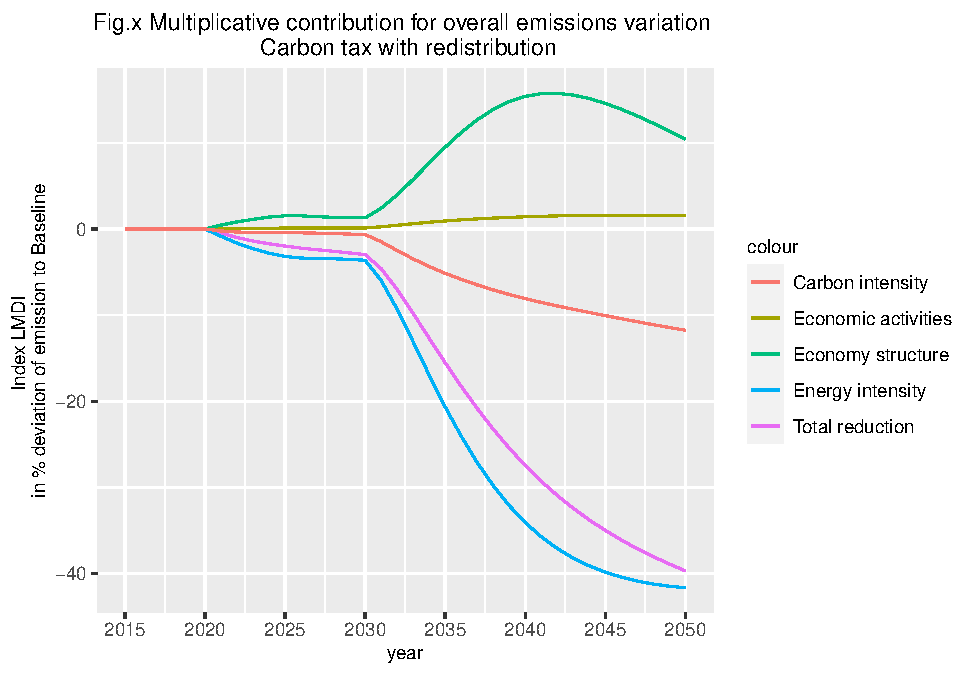
\includegraphics{Modele-ThreeMe-Tunisie_Sequeira_Valilou_Wang_files/figure-latex/unnamed-chunk-20-1.pdf}

Along with the economical growth, we find that the emissions reduction
of 42.2\% by 2050 is achieved, then we are now interested in its
pathway. To do this, we firstly employ our extended Kaya identity to
clarify the main driving forces, where, a priori, Economic activities
are expected to have positive effects on emissions, whilst Energy
intensity and Carbon intensity should have negative effects. Figure X.
presents the results of all the aggregated driving forces. We observe
that economy structure has a significantly positive and growing impact
until 2043 where it reaches the peak raising 7947.48 Kt CO2 (+19,38\%)
with regard to baseline, then it begins to decline to 5650,17 Kt CO2
(+12,46\%) on 2050. On the other hand, carbon intensity and energy
intensity show the negative and monotone trend, the former reducing
7128.35 Kt CO2 (-13.77\%) on 2050 and 30715.93 Kt CO2 (-47.18\%) for the
later. However, the influence of economic activities is negligible
(+886,37 Kt CO2 \& +1.86\%), revealing that even though the total
production remains relatively invariable, the revolution of economy
structure and production methods could still strongly impact the
emissions pathway.

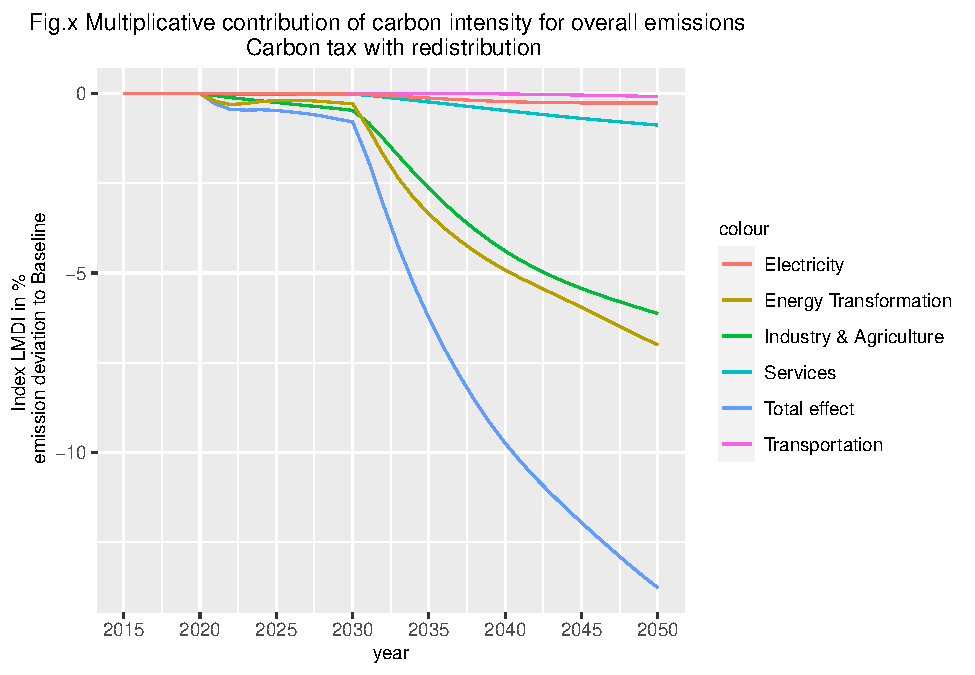
\includegraphics{Modele-ThreeMe-Tunisie_Sequeira_Valilou_Wang_files/figure-latex/unnamed-chunk-21-1.pdf}

So how do these driving forces work exactly to impact emissions? To
answer this question, we conduct a sectorial analysis with the help of
our extended Kaya identity. Fig.X depicts the evolution of economy
structure for different sectors. Electricity sector has a positive
impact while energy transformation has a negative one, with all other
sectors staying relatively stable. It indicates the development of
electricity production, and recession of another, standing for the
substitution of electricity over fossil fuels. Compared with fossil
fuels, electricity is potentially less pollutant because it is the final
conversion of renewable energies.

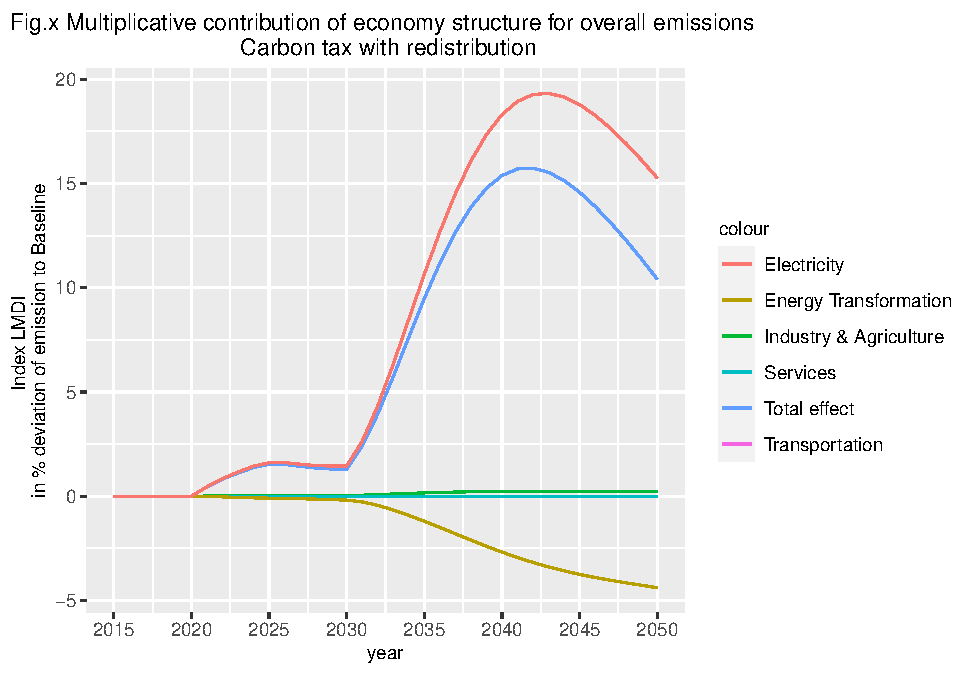
\includegraphics{Modele-ThreeMe-Tunisie_Sequeira_Valilou_Wang_files/figure-latex/unnamed-chunk-22-1.pdf}

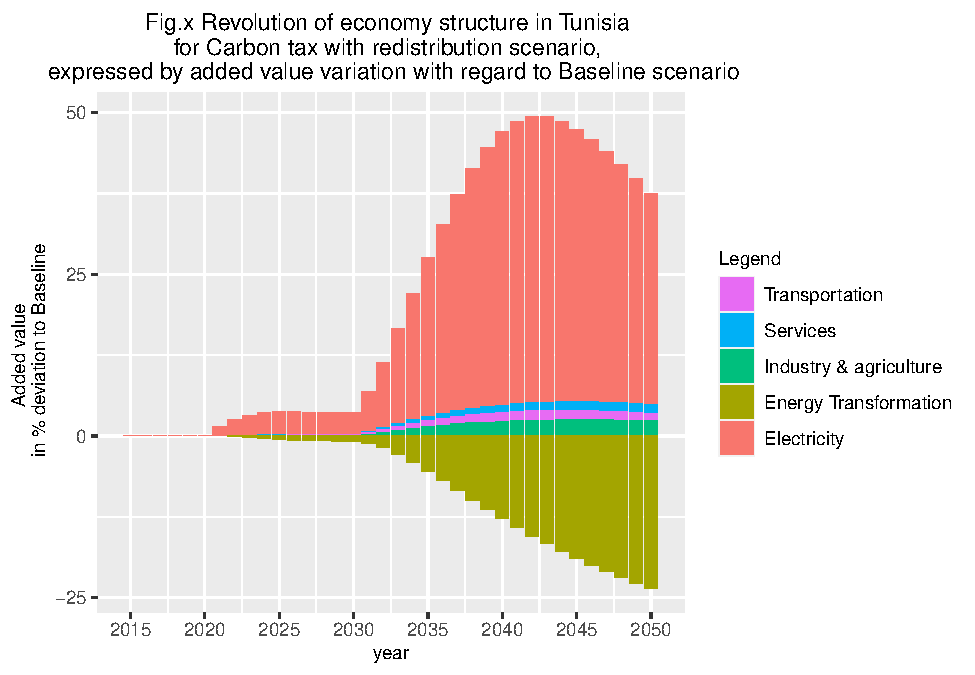
\includegraphics{Modele-ThreeMe-Tunisie_Sequeira_Valilou_Wang_files/figure-latex/unnamed-chunk-23-1.pdf}

The carbon tax induces the increasing investment for all sectors except
energy transformation, firstly to accelerate the penetration of
renewable energies in electricity mix and secondly, to reduce the
consumption of fossil fuels especially for energy intensive sectors. We
observe then the improvement of energy efficiency, in another word
reduction of energy intensity, for all the sectors of Tunisia's economy,
especially for electricity and industry \& agriculture (Fig.x). However,
the other sectors display slight reduction of energy intensity. For
example, the transportation sector consume majorly jet fuel for aircraft
and diesel for container ship. Electrification faces still huge
challenges for long distance transportation. The inertia of energy
demand thus exists in such a sector despite of the increasing cost for
carbon dioxide emission.

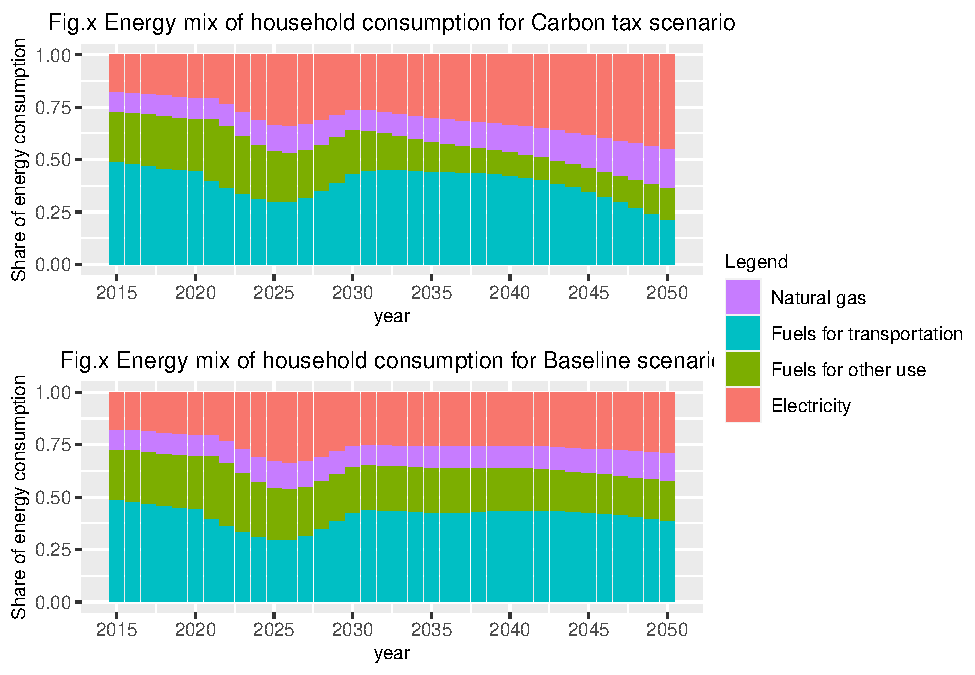
\includegraphics{Modele-ThreeMe-Tunisie_Sequeira_Valilou_Wang_files/figure-latex/unnamed-chunk-24-1.pdf}

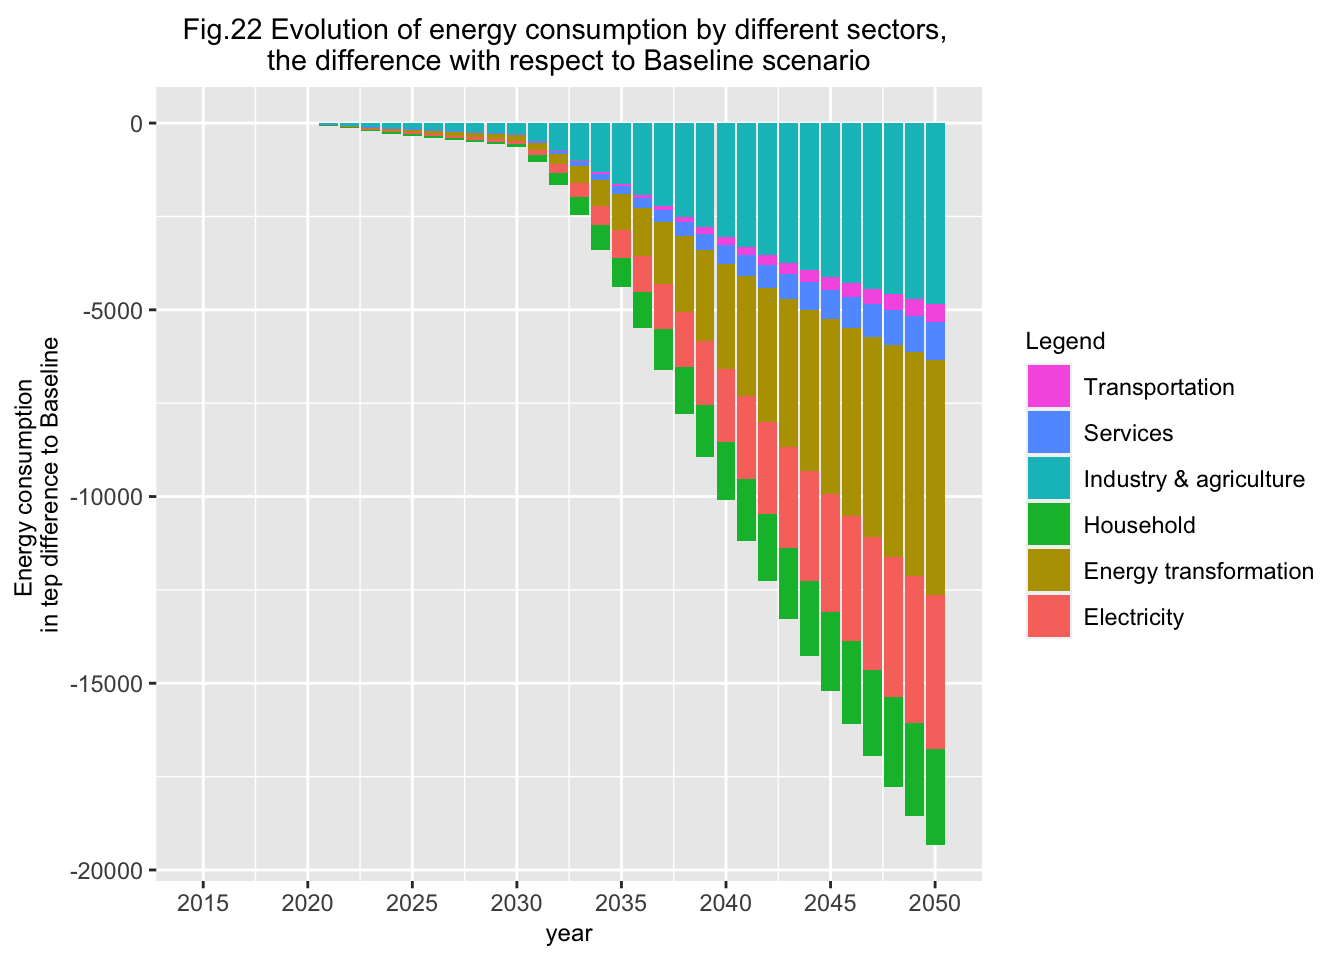
\includegraphics{Modele-ThreeMe-Tunisie_Sequeira_Valilou_Wang_files/figure-latex/unnamed-chunk-25-1.pdf}

Fig.x shows how energy consumption varies with the carbon tax, which can
be explained by improvement of energy intensity. As what we discussed
above, we can find more and more diminished energy demand for all the
economic sectors and for household. And one more time, we observe the
inertia for transportation and services. Even though there is not
noticeable amelioration of energy intensity for energy transformation,
the overall shrinkage of the sector explains the energy demand profile.

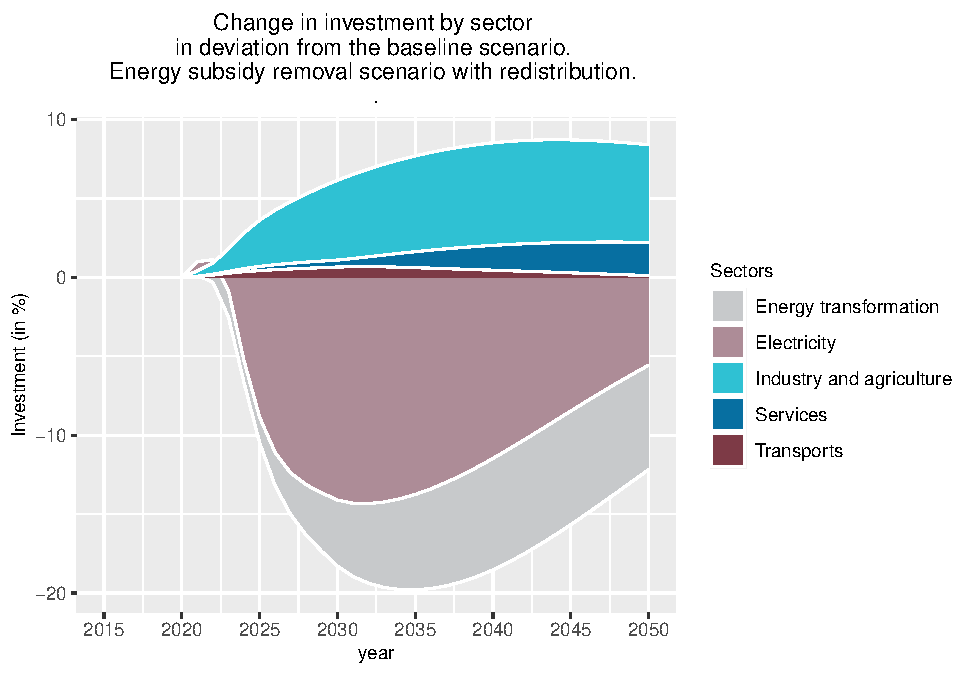
\includegraphics{Modele-ThreeMe-Tunisie_Sequeira_Valilou_Wang_files/figure-latex/unnamed-chunk-26-1.pdf}

The energy intensity represents the choice of production technology
considering whether it is energy intensive or not, whilst the carbon
intensity describes how carbon tax leads the economy to choose the types
of energy. We notice a moderate fall for industry \& agriculture and
energy transformation, meaning the transition towards energies with less
emission. The electricity mix is exogenous according to our modelling
assumptions, that is why the carbon tax has no effect on it, whereas it
might be wildly influenced by climate policies in the real situation. It
is worthy to mention here that energy consumption by household are
almost from energy transformation sector, so we integrated household
energy consumption into energy transformation sector. In fact, the
reduction of carbon intensity observed here in energy transformation
sector is arose by a different energy mix of household rather than the
sector itself.

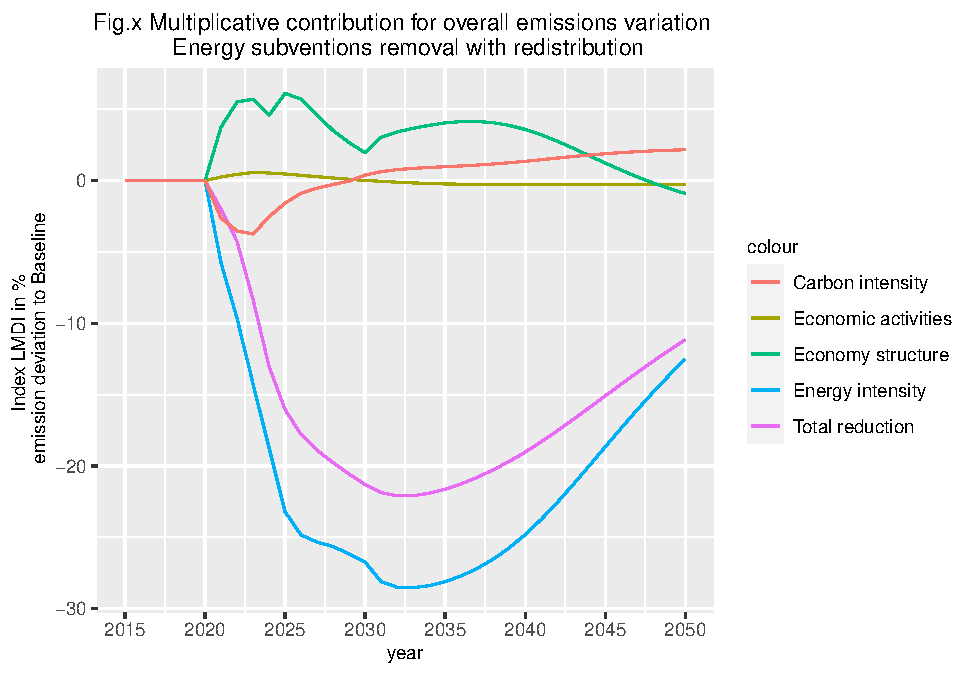
\includegraphics{Modele-ThreeMe-Tunisie_Sequeira_Valilou_Wang_files/figure-latex/unnamed-chunk-27-1.pdf}

As the carbon tax induces the production of green electricity (with less
pollution per unit of energy production), the energy consumers then have
a more environmental friendly alternative other than fuel. Even though
maybe they are not intended to care about the climate change, using this
alternative enables them to cut back their costs. Therefore, we see the
rapid shifting from fossil fuel to electricity for industry \&
agriculture and the household, and reaching nearly a half of their
energy consumption until 2050 like depicted in Fig.X to X. For industry
\& agriculture, electricity mainly offsets a part of natural gas demand,
which hints the electrification of heating unit for instance. As for
household, the wild spread of electrical or hybrid cars reduces the
domand for fossil fuel.

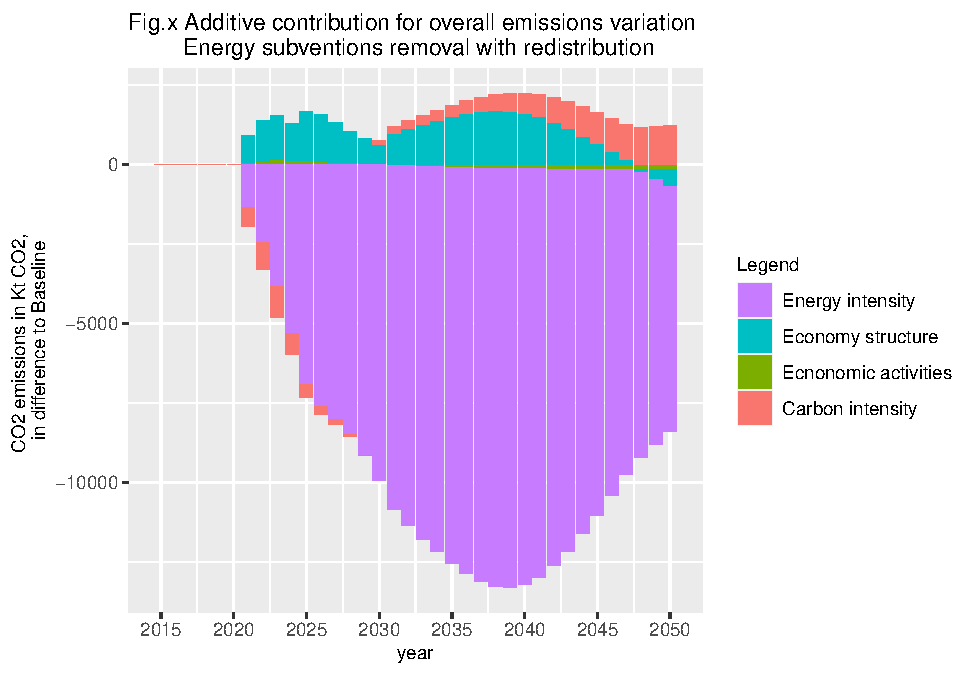
\includegraphics{Modele-ThreeMe-Tunisie_Sequeira_Valilou_Wang_files/figure-latex/unnamed-chunk-28-1.pdf}

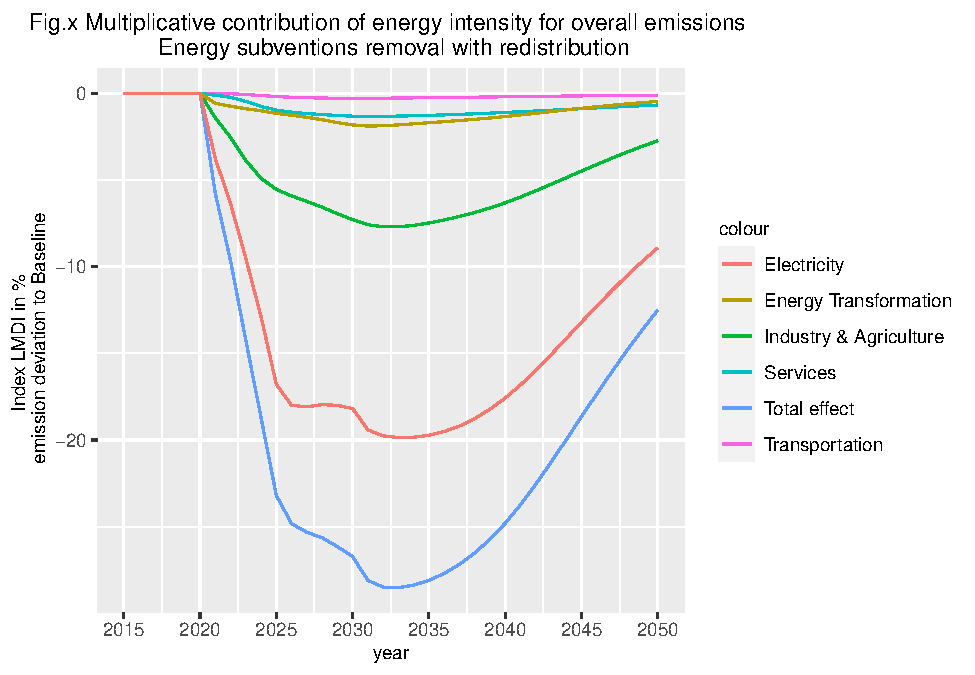
\includegraphics{Modele-ThreeMe-Tunisie_Sequeira_Valilou_Wang_files/figure-latex/unnamed-chunk-29-1.pdf}

\hypertarget{energy-subsidies-removal-bee}{%
\subsection{Energy subsidies removal
(bee)}\label{energy-subsidies-removal-bee}}

\hypertarget{economic-impacts}{%
\subsubsection{Economic impacts}\label{economic-impacts}}

\begin{longtabu} to \linewidth {>{\raggedright}X>{\raggedleft}X>{\raggedleft}X>{\raggedleft}X>{\raggedleft}X>{\raggedleft}X>{\raggedleft}X>{\raggedleft}X}
\caption{\label{tab:unnamed-chunk-30}Macroeconomic impacts of Energy subsidies removal }\\
\toprule
\textbf{ } & \textbf{2021} & \textbf{2025} & \textbf{2030} & \textbf{2035} & \textbf{2040} & \textbf{2045} & \textbf{2050}\\
\midrule
\endfirsthead
\caption[]{Macroeconomic impacts of Energy subsidies removal  \textit{(continued)}}\\
\toprule
\textbf{ } & \textbf{2021} & \textbf{2025} & \textbf{2030} & \textbf{2035} & \textbf{2040} & \textbf{2045} & \textbf{2050}\\
\midrule
\endhead

\endfoot
\bottomrule
\endlastfoot
\cellcolor{gray!6}{GDP in volume} & \cellcolor{gray!6}{0.17} & \cellcolor{gray!6}{0.56} & \cellcolor{gray!6}{0.32} & \cellcolor{gray!6}{0.13} & \cellcolor{gray!6}{0.06} & \cellcolor{gray!6}{0.01} & \cellcolor{gray!6}{-0.03}\\
Household consumption & -0.02 & 0.06 & 0.10 & 0.39 & 0.63 & 0.72 & 0.68\\
\cellcolor{gray!6}{Investment} & \cellcolor{gray!6}{0.16} & \cellcolor{gray!6}{-0.19} & \cellcolor{gray!6}{-0.49} & \cellcolor{gray!6}{0.20} & \cellcolor{gray!6}{1.01} & \cellcolor{gray!6}{1.68} & \cellcolor{gray!6}{2.10}\\
Exports & 0.00 & -0.22 & -0.94 & -1.58 & -1.85 & -1.84 & -1.71\\
\cellcolor{gray!6}{Imports} & \cellcolor{gray!6}{-0.30} & \cellcolor{gray!6}{-1.22} & \cellcolor{gray!6}{-1.34} & \cellcolor{gray!6}{-0.86} & \cellcolor{gray!6}{-0.28} & \cellcolor{gray!6}{0.27} & \cellcolor{gray!6}{0.65}\\
Household disposable income & -0.01 & 0.05 & 0.09 & 0.40 & 0.62 & 0.71 & 0.68\\
\cellcolor{gray!6}{Household consumption price index} & \cellcolor{gray!6}{0.27} & \cellcolor{gray!6}{2.13} & \cellcolor{gray!6}{3.88} & \cellcolor{gray!6}{4.59} & \cellcolor{gray!6}{4.62} & \cellcolor{gray!6}{4.25} & \cellcolor{gray!6}{3.81}\\
Real cost of labor & 0.56 & 2.19 & 1.43 & 0.43 & -0.03 & -0.33 & -0.53\\
\cellcolor{gray!6}{Unemployment rate (in point)} & \cellcolor{gray!6}{-0.07} & \cellcolor{gray!6}{-0.30} & \cellcolor{gray!6}{0.04} & \cellcolor{gray!6}{0.18} & \cellcolor{gray!6}{0.11} & \cellcolor{gray!6}{-0.03} & \cellcolor{gray!6}{-0.15}\\
Trade balance (in point of GDP) & 0.39 & 2.57 & 2.99 & 2.31 & 1.60 & 1.03 & 0.65\\
\cellcolor{gray!6}{Public budget balance (in points of GDP)} & \cellcolor{gray!6}{0.24} & \cellcolor{gray!6}{1.83} & \cellcolor{gray!6}{2.41} & \cellcolor{gray!6}{2.08} & \cellcolor{gray!6}{1.61} & \cellcolor{gray!6}{1.11} & \cellcolor{gray!6}{0.73}\\
Public debt (in points of GDP) & -0.50 & -6.41 & -15.82 & -22.39 & -25.38 & -26.20 & -25.56\\
\cellcolor{gray!6}{CO2 emissions} & \cellcolor{gray!6}{-3.63} & \cellcolor{gray!6}{-17.01} & \cellcolor{gray!6}{-20.74} & \cellcolor{gray!6}{-20.34} & \cellcolor{gray!6}{-17.53} & \cellcolor{gray!6}{-13.49} & \cellcolor{gray!6}{-9.66}\\*
\end{longtabu}

Table.X : Macroeconomic impacts of Energy subsidies removal scenario in
\% deviation to Baseline!

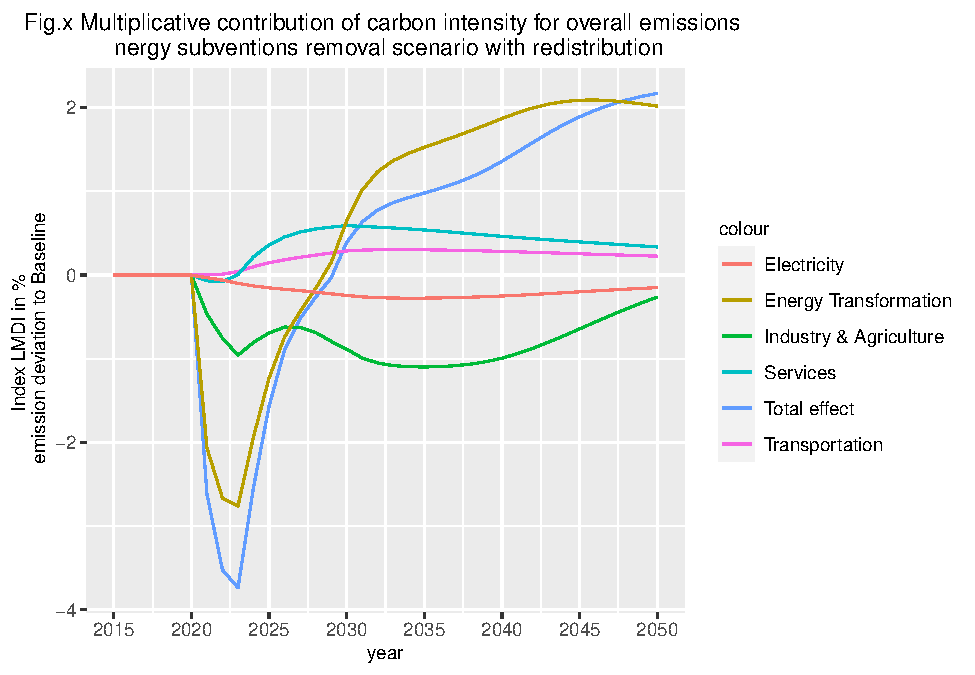
\includegraphics{Modele-ThreeMe-Tunisie_Sequeira_Valilou_Wang_files/figure-latex/unnamed-chunk-32-1.pdf}

\hypertarget{environmental-and-energy-impacts}{%
\subsubsection{Environmental and energy
impacts}\label{environmental-and-energy-impacts}}

\begin{Shaded}
\begin{Highlighting}[]
\FunctionTok{ggplot}\NormalTok{() }\SpecialCharTok{+} 
  \FunctionTok{geom\_line}\NormalTok{(}\FunctionTok{aes}\NormalTok{(}\AttributeTok{x =}\NormalTok{ S4[,}\StringTok{"year"}\NormalTok{],}\AttributeTok{y =}\NormalTok{ S4[,}\StringTok{"ems\_co2\_2"}\NormalTok{]}\SpecialCharTok{/}\NormalTok{Baseline[,}\StringTok{"ems\_co2\_0"}\NormalTok{], }\AttributeTok{group =} \DecValTok{1}\NormalTok{, }\AttributeTok{color =} \StringTok{"Total effect"}\NormalTok{), }\AttributeTok{size =} \FloatTok{1.0}\NormalTok{) }\SpecialCharTok{+} 
  \FunctionTok{geom\_line}\NormalTok{(}\FunctionTok{aes}\NormalTok{(}\AttributeTok{x =}\NormalTok{ S4[,}\StringTok{"year"}\NormalTok{],}\AttributeTok{y =}\NormalTok{ S4[,}\StringTok{"va\_2"}\NormalTok{]}\SpecialCharTok{/}\NormalTok{Baseline[,}\StringTok{"va\_0"}\NormalTok{], }\AttributeTok{group =} \DecValTok{1}\NormalTok{, }\AttributeTok{color =} \StringTok{"GDP per capita"}\NormalTok{)) }\SpecialCharTok{+} 
  \FunctionTok{geom\_line}\NormalTok{(}\FunctionTok{aes}\NormalTok{(}\AttributeTok{x =}\NormalTok{ S4[,}\StringTok{"year"}\NormalTok{],}\AttributeTok{y =}\NormalTok{ ((S4[,}\StringTok{"ci\_toe\_2"}\NormalTok{]}\SpecialCharTok{+}\NormalTok{S4[,}\StringTok{"ch\_toe\_2"}\NormalTok{])}\SpecialCharTok{/}\NormalTok{(Baseline[,}\StringTok{"ci\_toe\_0"}\NormalTok{]}\SpecialCharTok{+}\NormalTok{Baseline[,}\StringTok{"ch\_toe\_0"}\NormalTok{]))}\SpecialCharTok{/}\NormalTok{(S4[,}\StringTok{"va\_2"}\NormalTok{]}\SpecialCharTok{/}\NormalTok{Baseline[,}\StringTok{"va\_0"}\NormalTok{]), }\AttributeTok{group =} \DecValTok{1}\NormalTok{, }\AttributeTok{color =} \StringTok{"Energy intensity"}\NormalTok{)) }\SpecialCharTok{+} 
  \FunctionTok{geom\_line}\NormalTok{(}\FunctionTok{aes}\NormalTok{(}\AttributeTok{x =}\NormalTok{ S4[,}\StringTok{"year"}\NormalTok{],}\AttributeTok{y =}\NormalTok{  (S4[,}\StringTok{"ems\_co2\_2"}\NormalTok{]}\SpecialCharTok{/}\NormalTok{Baseline[,}\StringTok{"ems\_co2\_0"}\NormalTok{])}\SpecialCharTok{/}\NormalTok{((S4[,}\StringTok{"ci\_toe\_2"}\NormalTok{]}\SpecialCharTok{+}\NormalTok{S4[,}\StringTok{"ch\_toe\_2"}\NormalTok{])}\SpecialCharTok{/}\NormalTok{(Baseline[,}\StringTok{"ci\_toe\_0"}\NormalTok{]}\SpecialCharTok{+}\NormalTok{Baseline[,}\StringTok{"ch\_toe\_0"}\NormalTok{])), }\AttributeTok{group =} \DecValTok{1}\NormalTok{, }\AttributeTok{color =} \StringTok{"Carbon Intensity"}\NormalTok{)) }\SpecialCharTok{+} 
  \FunctionTok{labs}\NormalTok{(}\AttributeTok{x =} \StringTok{"year"}\NormalTok{, }\AttributeTok{y =} \StringTok{"Index of Kaya identity"}\NormalTok{, }\AttributeTok{title =} \StringTok{"Kaya identity at aggragated level }\SpecialCharTok{\textbackslash{}n}\StringTok{Energy subsidy with redistribution scenario"}\NormalTok{) }\SpecialCharTok{+}
  \FunctionTok{scale\_x\_continuous}\NormalTok{(}\AttributeTok{breaks=}\FunctionTok{seq}\NormalTok{(}\DecValTok{2015}\NormalTok{,}\DecValTok{2050}\NormalTok{,}\DecValTok{5}\NormalTok{))}
\end{Highlighting}
\end{Shaded}

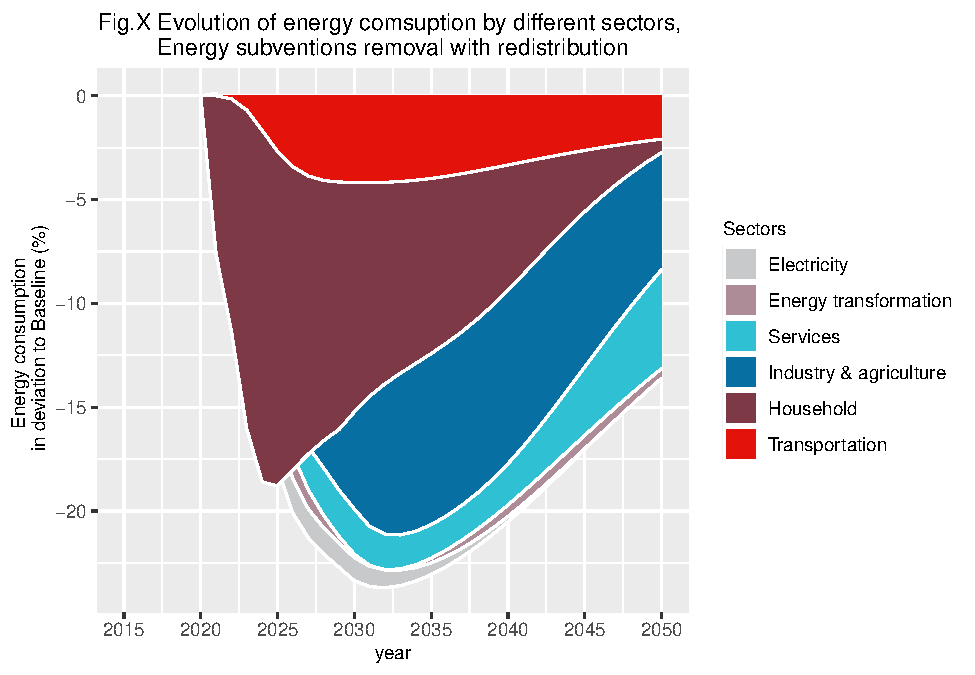
\includegraphics{Modele-ThreeMe-Tunisie_Sequeira_Valilou_Wang_files/figure-latex/unnamed-chunk-33-1.pdf}

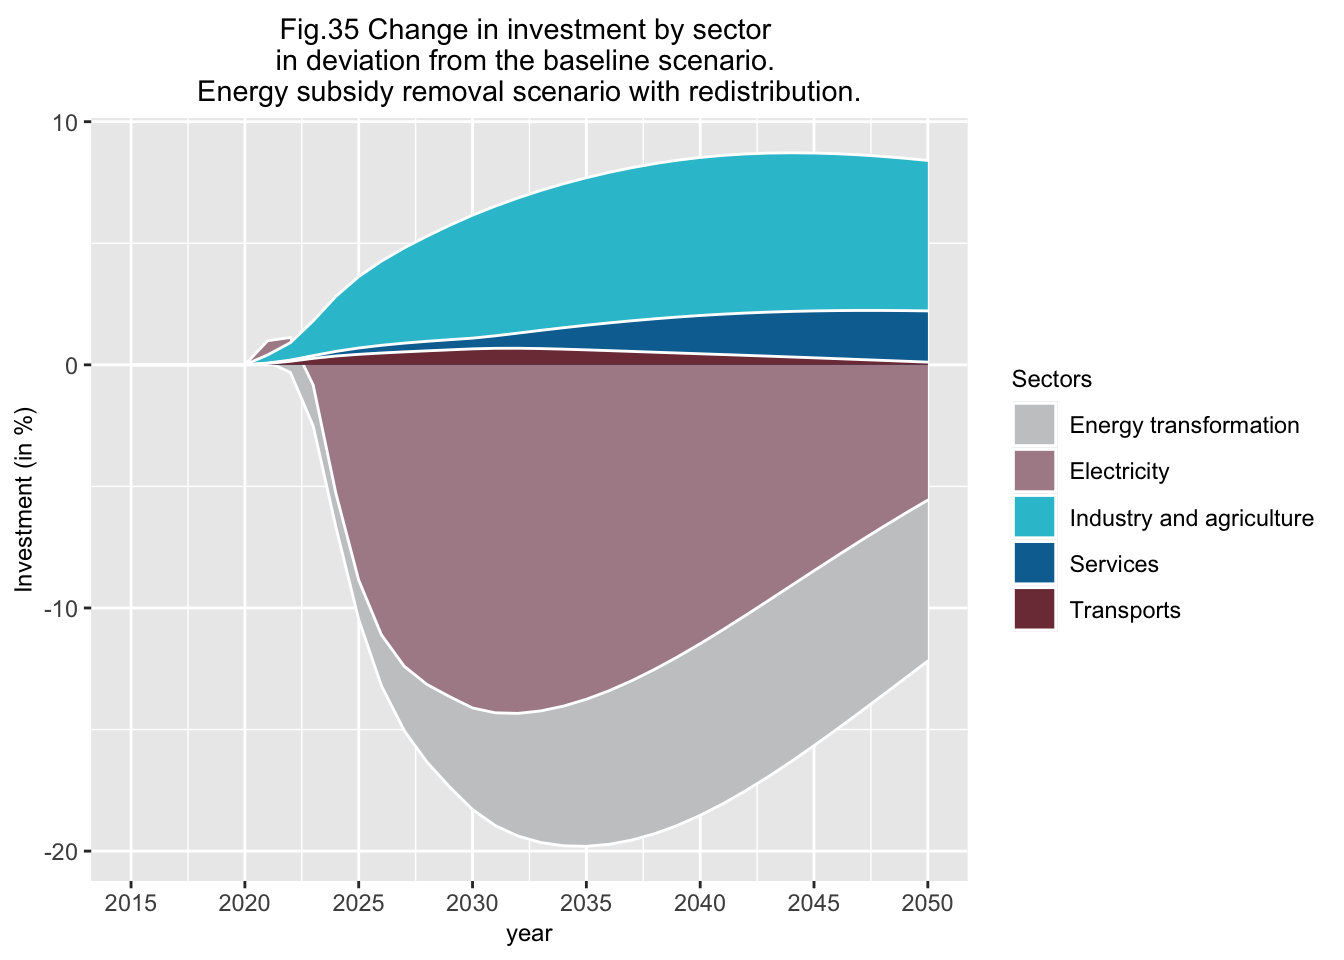
\includegraphics{Modele-ThreeMe-Tunisie_Sequeira_Valilou_Wang_files/figure-latex/unnamed-chunk-34-1.pdf}

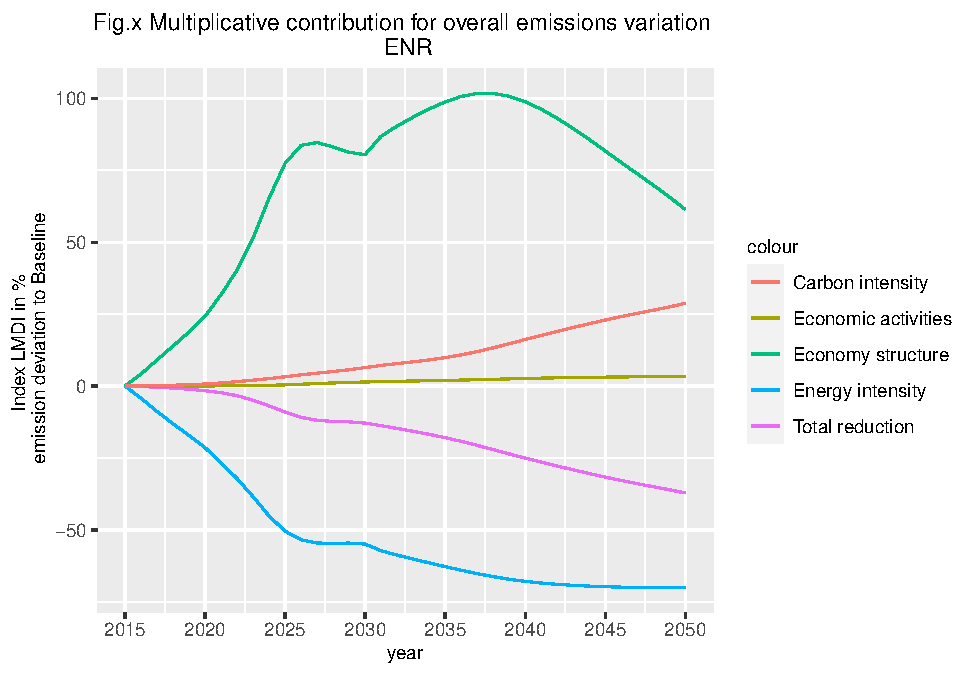
\includegraphics{Modele-ThreeMe-Tunisie_Sequeira_Valilou_Wang_files/figure-latex/unnamed-chunk-35-1.pdf}

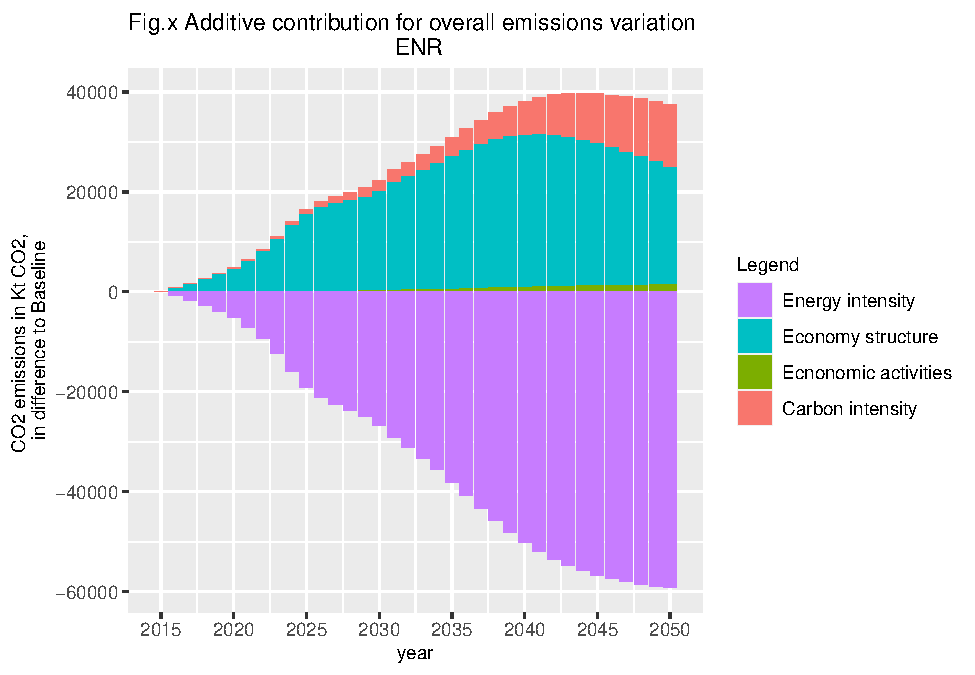
\includegraphics{Modele-ThreeMe-Tunisie_Sequeira_Valilou_Wang_files/figure-latex/unnamed-chunk-36-1.pdf}

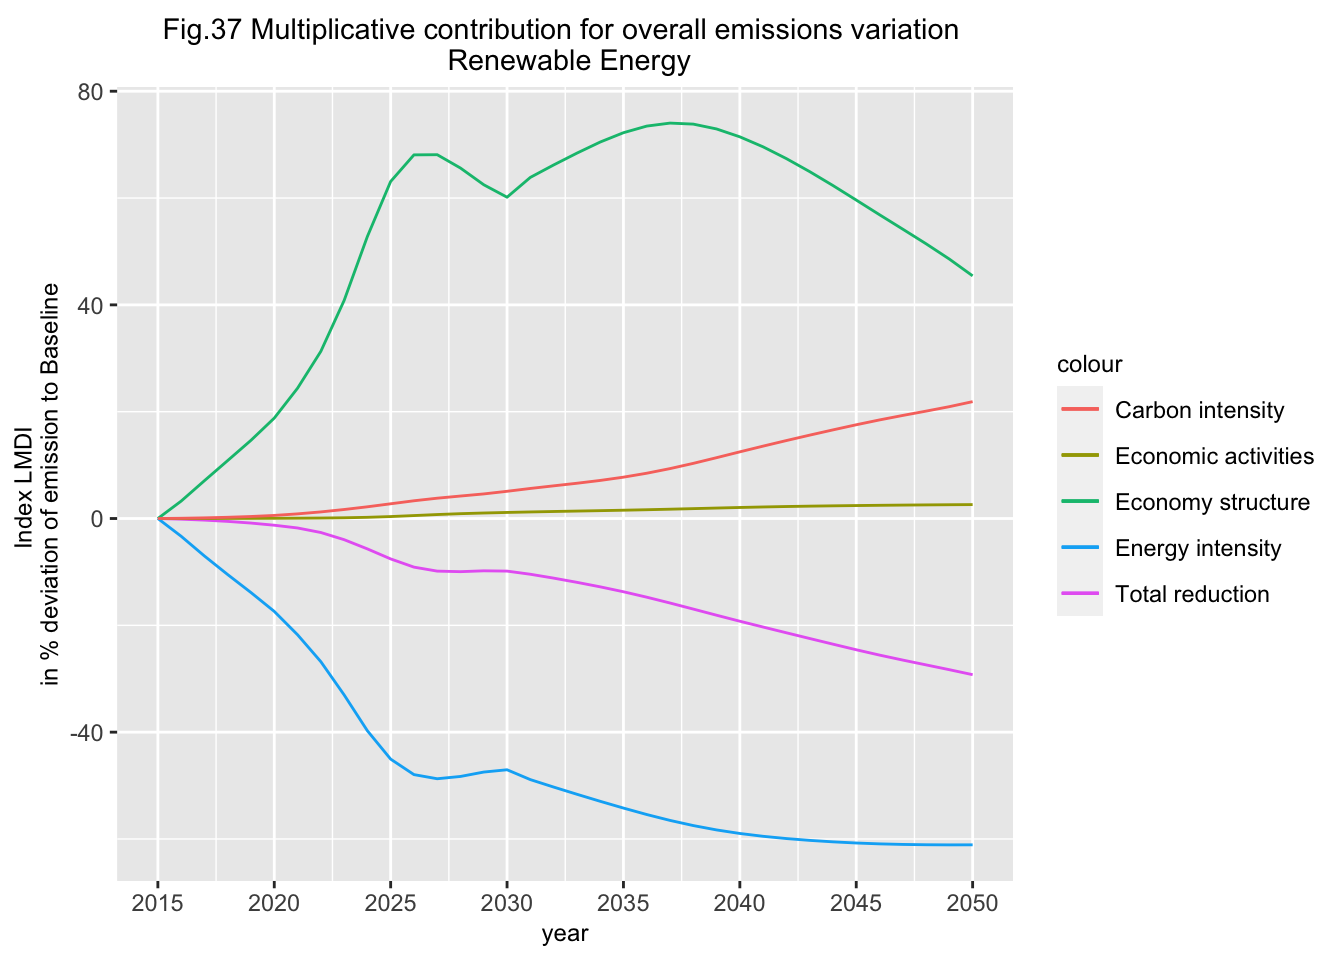
\includegraphics{Modele-ThreeMe-Tunisie_Sequeira_Valilou_Wang_files/figure-latex/unnamed-chunk-37-1.pdf}
\includegraphics{Modele-ThreeMe-Tunisie_Sequeira_Valilou_Wang_files/figure-latex/unnamed-chunk-37-2.pdf}

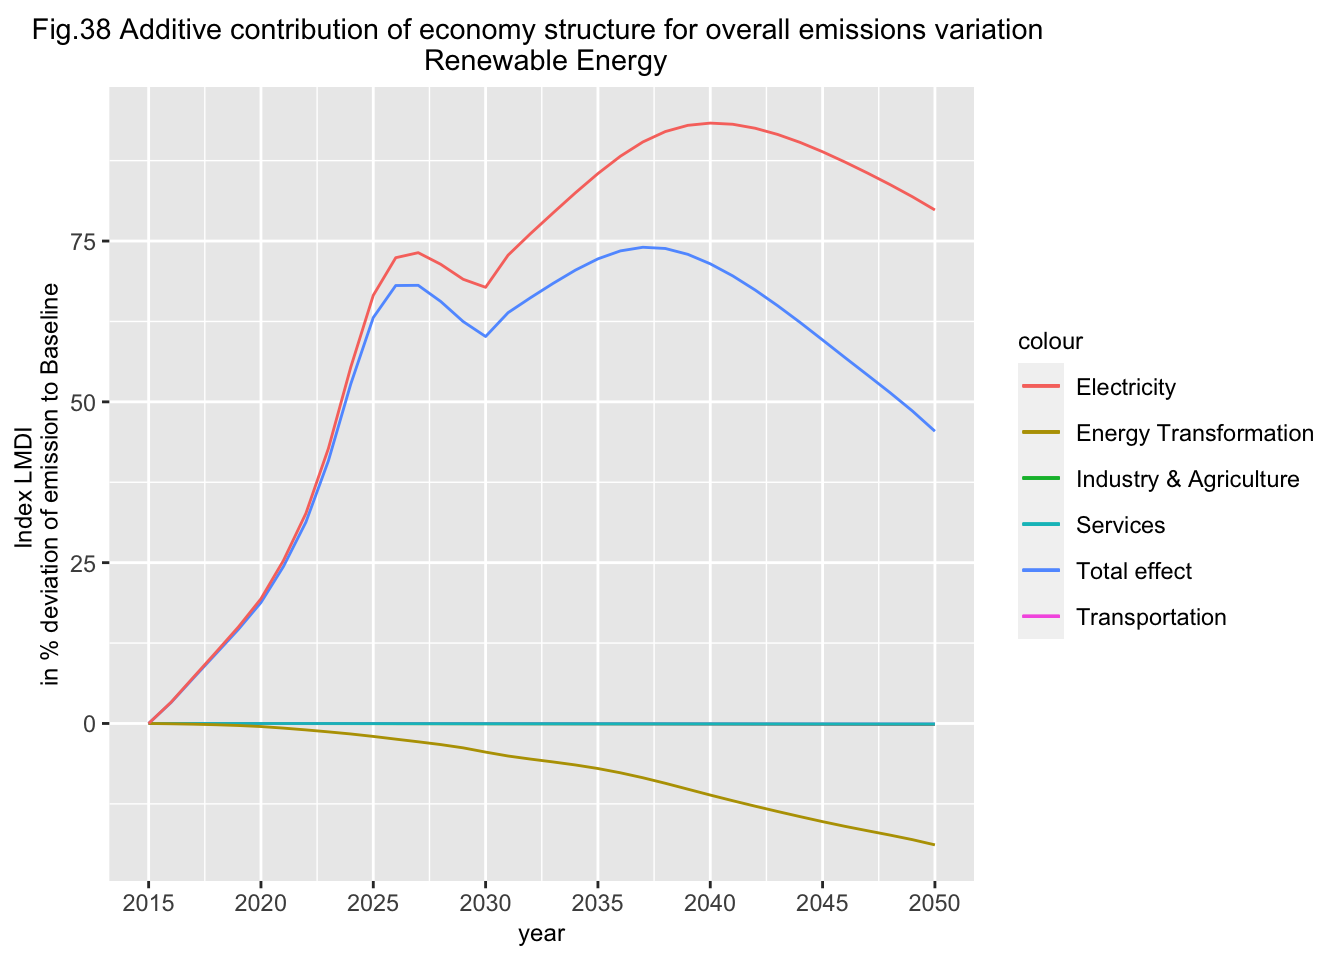
\includegraphics{Modele-ThreeMe-Tunisie_Sequeira_Valilou_Wang_files/figure-latex/unnamed-chunk-38-1.pdf}

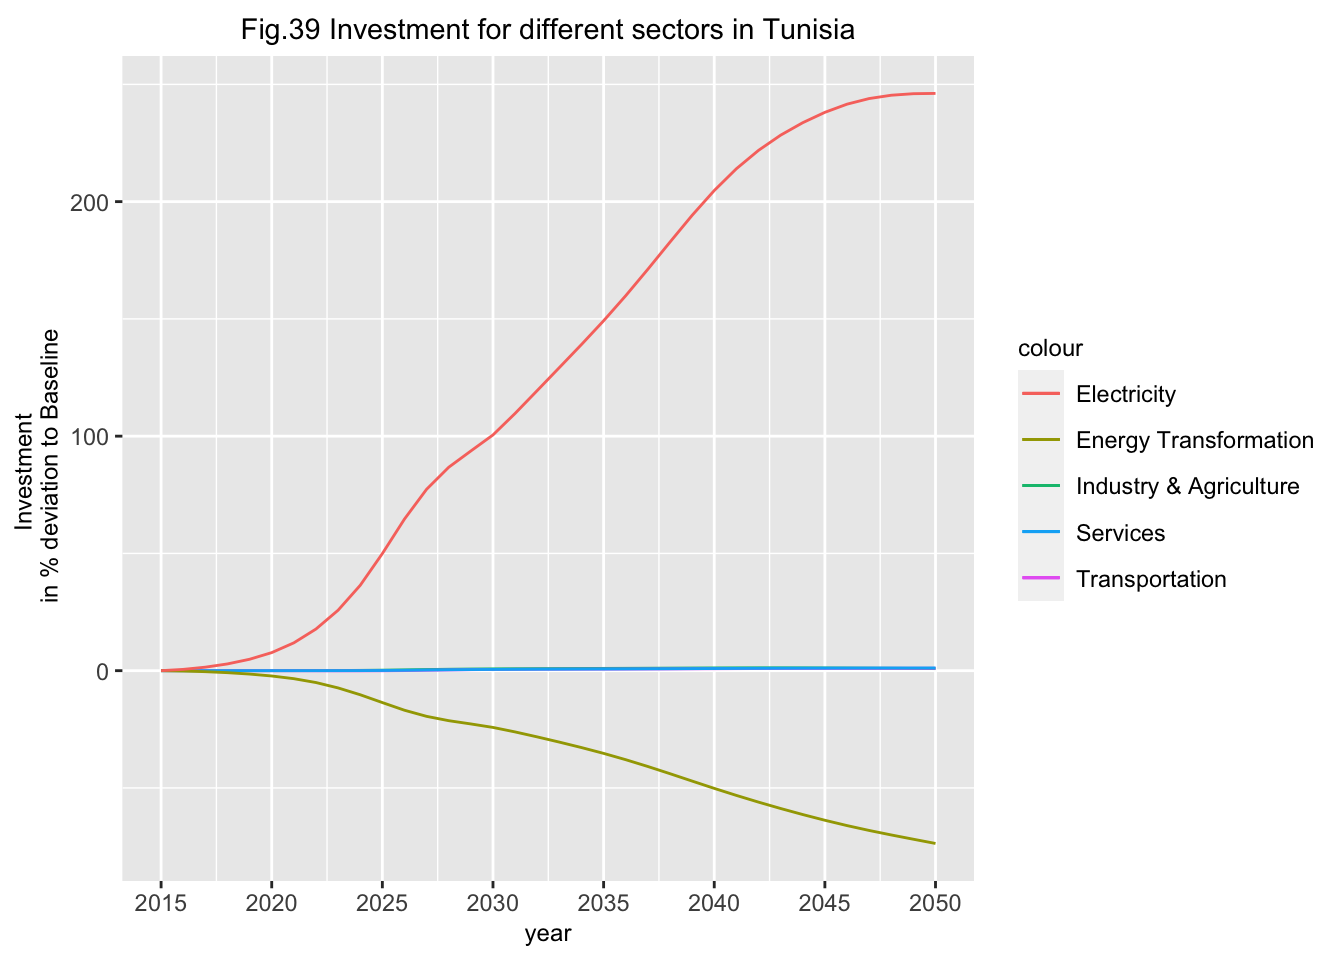
\includegraphics{Modele-ThreeMe-Tunisie_Sequeira_Valilou_Wang_files/figure-latex/unnamed-chunk-39-1.pdf}

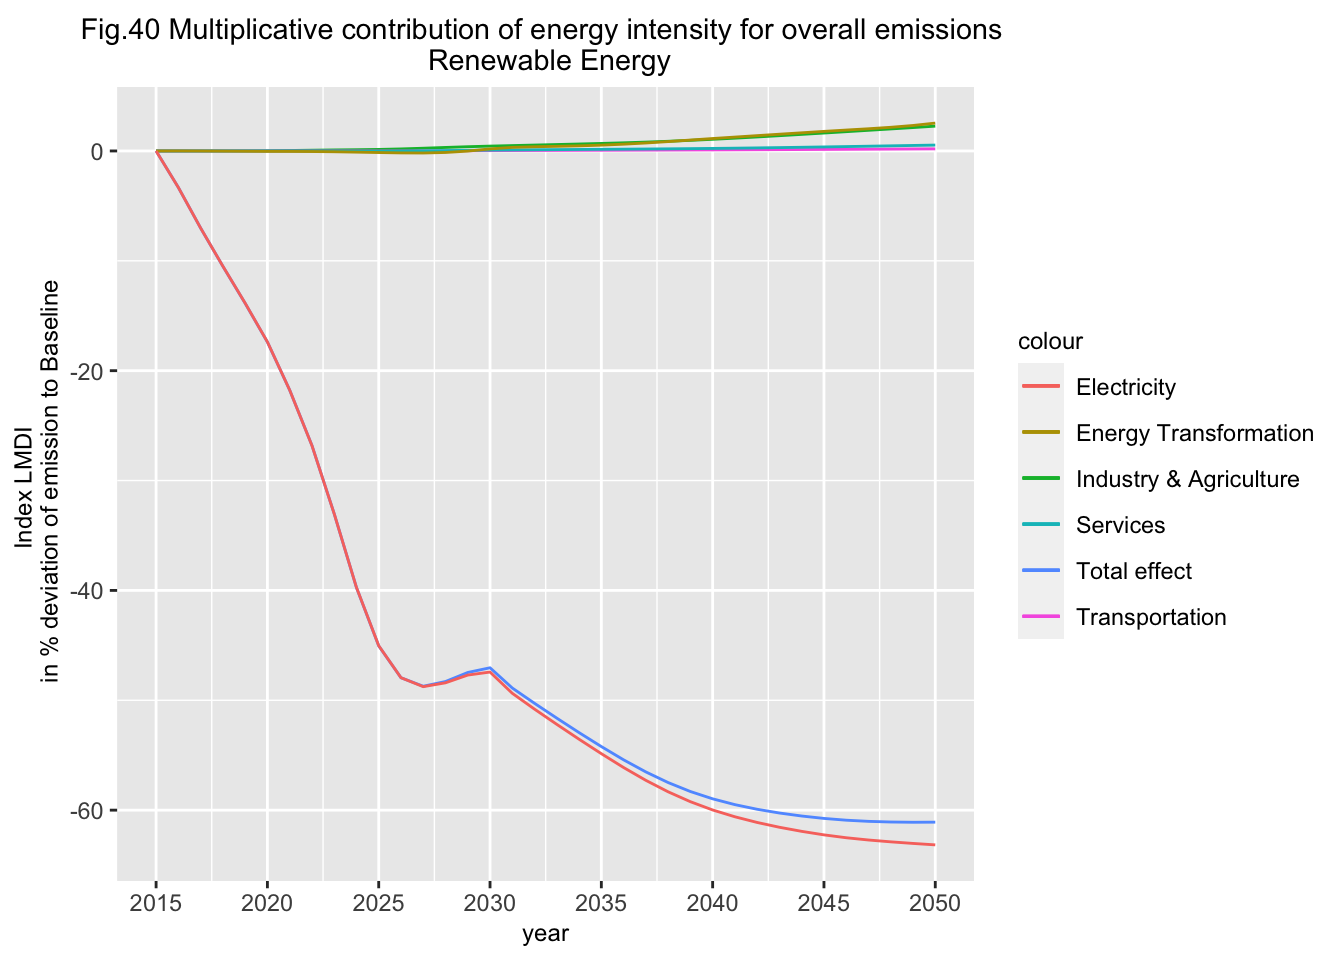
\includegraphics{Modele-ThreeMe-Tunisie_Sequeira_Valilou_Wang_files/figure-latex/unnamed-chunk-40-1.pdf}

\hypertarget{renewable-energy-scenario-1}{%
\subsection{Renewable energy
scenario}\label{renewable-energy-scenario-1}}

Table.X :Macroeconomic impacts of Energy subsidies removal scenario in
\% deviation to Baseline

\includegraphics{Modele-ThreeMe-Tunisie_Sequeira_Valilou_Wang_files/figure-latex/unnamed-chunk-42-1.pdf}

\includegraphics{Modele-ThreeMe-Tunisie_Sequeira_Valilou_Wang_files/figure-latex/unnamed-chunk-43-1.pdf}

\includegraphics{Modele-ThreeMe-Tunisie_Sequeira_Valilou_Wang_files/figure-latex/unnamed-chunk-44-1.pdf}

\includegraphics{Modele-ThreeMe-Tunisie_Sequeira_Valilou_Wang_files/figure-latex/unnamed-chunk-45-1.pdf}

\includegraphics{Modele-ThreeMe-Tunisie_Sequeira_Valilou_Wang_files/figure-latex/unnamed-chunk-46-1.pdf}

\includegraphics{Modele-ThreeMe-Tunisie_Sequeira_Valilou_Wang_files/figure-latex/unnamed-chunk-47-1.pdf}

\includegraphics{Modele-ThreeMe-Tunisie_Sequeira_Valilou_Wang_files/figure-latex/unnamed-chunk-48-1.pdf}

\includegraphics{Modele-ThreeMe-Tunisie_Sequeira_Valilou_Wang_files/figure-latex/unnamed-chunk-49-1.pdf}

\includegraphics{Modele-ThreeMe-Tunisie_Sequeira_Valilou_Wang_files/figure-latex/unnamed-chunk-50-1.pdf}

\hypertarget{national-low-carbon-strategy-scenario-1}{%
\subsection{National Low-Carbon Strategy
scenario}\label{national-low-carbon-strategy-scenario-1}}

Table.X :Macroeconomic impacts of Nation Low-Carbon Strategy scenario in
\% deviation to Baseline

\includegraphics{Modele-ThreeMe-Tunisie_Sequeira_Valilou_Wang_files/figure-latex/unnamed-chunk-52-1.pdf}

\includegraphics{Modele-ThreeMe-Tunisie_Sequeira_Valilou_Wang_files/figure-latex/unnamed-chunk-53-1.pdf}

\includegraphics{Modele-ThreeMe-Tunisie_Sequeira_Valilou_Wang_files/figure-latex/unnamed-chunk-54-1.pdf}

\includegraphics{Modele-ThreeMe-Tunisie_Sequeira_Valilou_Wang_files/figure-latex/unnamed-chunk-55-1.pdf}

\includegraphics{Modele-ThreeMe-Tunisie_Sequeira_Valilou_Wang_files/figure-latex/unnamed-chunk-56-1.pdf}

\includegraphics{Modele-ThreeMe-Tunisie_Sequeira_Valilou_Wang_files/figure-latex/unnamed-chunk-57-1.pdf}

\includegraphics{Modele-ThreeMe-Tunisie_Sequeira_Valilou_Wang_files/figure-latex/unnamed-chunk-58-1.pdf}

\includegraphics{Modele-ThreeMe-Tunisie_Sequeira_Valilou_Wang_files/figure-latex/unnamed-chunk-59-1.pdf}

\hypertarget{prolongements}{%
\section{Prolongements}\label{prolongements}}

\hypertarget{dautres-leviers-pour-analyser-ouverture}{%
\subsection{D'autres leviers pour analyser
(ouverture)}\label{dautres-leviers-pour-analyser-ouverture}}

\hypertarget{lamuxe9lioration-du-cadre-statistique}{%
\subsection{L'amélioration du cadre
statistique}\label{lamuxe9lioration-du-cadre-statistique}}

OUverture : pb du secteur informel non pris en compte par la
comptabilité nationale

\hypertarget{conclusion}{%
\section{Conclusion}\label{conclusion}}

\printbibliography[title=Bibliographie]

\end{document}
